\documentclass[12pt,a4paper]{report}
\usepackage{graphicx}
\usepackage{tabularx}
\usepackage{array}

\begin{document}
%--------------Title Page ------------------
\thispagestyle{empty}
\begin{center}
\textbf{\large{Merchant Monetary System}}\\
\vspace{0.5cm}
\textbf{ CS-262 Design Document} \\
\vspace{1.5cm}

\includegraphics[scale=.07]{UETLogo}\\
\vspace{1.5cm}
\underline{ Project Supervisor}\\
\vspace{0.5cm}
Mr. Samyan Qayyum Wahla\\
\vspace{1cm}
\underline {Group ID $(G 11)$} \\
\vspace{0.5cm}
Project Member\\
\vspace{0.5cm}
\begin{tabular}{ m{5cm} m{4cm}}
 Syed Hashir & 2021-CS-1 \\ 
 Kabir Ahmed & 2021-CS-4  \\  
 M. Hamad Hassan & 2021-CS-33
\end{tabular}
\vspace{2cm}
\par\rule{\textwidth}{0.5pt} 
Department of Computer Science\\
University of Engineering and Technology, Lahore\\
Pakistan
\end{center}
\newpage

\tableofcontents
\thispagestyle{empty}
\pagenumbering{arabic}


\newpage
\setcounter{page}{1}
\chapter {Project Description}

The system is designed for a company that provides
logistics (delivery of products to its client), product management (crud operations), and effective communication with their worker, clients, and vendors.
 
The company has its office, warehouse, and rider. 
It has a different contract with multiple firms to take the shipment from the vendors and store it in dedicated warehouses. The rider will take orders from the shopkeeper. Their order is received at the office, and the office will create the feasibility report according to their shopkeepers' needs and instructions generated for their warehouse manager to fulfill their order. The area-specific rider will receive an email about their order. The office will send a confirmation email to their shopkeeper. 
 
There are a total of four actors in the system and two stakeholders. Their titles and roles are:
\begin{itemize}
\item \textbf{ CEO:} The company's owner manages all the operations.
\item \textbf{Employee:} They are assistants to CEO to help in company operations. 
\item \textbf{Warehouse Manager:} Received the instructions from the employee and ready the shipment for the rider, and managed other expenses.
\item \textbf{Rider:} They take orders from different shopkeepers and deliver the product according to pre-subscribed routes defined by the system.
\end{itemize}
The stakeholder is:
\begin{itemize}
\item \textbf{Shopkeepers:} Getting the goods and services from the company.
\item \textbf{Vendor:} The vendor will provide the products to the company. 
\end{itemize}
This system is designed for one company and one CEO. CEO will be provided with already defined credentials. The CEO is responsible for creating accounts for all others actors. The CEO will provide a credential to the actors, and they will be able to update their credentials. 
 
The first dedicated dashboard for the CEO, where they monitor all operations. The operations manage their workers, products, and expenses and send emails. The CEO is the only person in the system with access to all operations. CEO analyzes company operations, including the performance of their workers and inventory. The system will present the company expenditure report.
 
The second dashboard is for office employees. They have access to manage emails, shopkeepers' orders, vendors' shipments, and company expenses. The company's expenses are the CEO, rider, and warehouse salaries. The system will present the report of payment to the vendor and shopkeeper. An employee will enter all the shipments that the company receives. They add product identifiers.
 
The third dashboard is for the warehouse manager, who receives feasibility reports of office employees and prepares the order for the rider. The warehouse manager must record the labor used in preparing the order. It could provide the miscellaneous expenses of the warehouse, like electricity costs, etc. They can view the product and make suitable changes according to the requirements.
 
The fourth dashboard is for a rider, which is basically the communicator between the company and the shopkeeper.
The rider is responsible for taking orders from the shopkeeper. 
Enter order details into the system. 
The riders will check the current orders assigned to them by the company. They will pick up the shipment from the warehouse and delivery them to the shopkeeper. The system will present the routes to the destination with the order detail. The rider received a specific amount of fuel to perform the operations. The prescribed fuel is calculated according to the formula. They can see all the products. The product will be sorted in any order. Search for a specific product from a wide range of available products. The system will deploy different sharp algorithms to access the desired date orders quickly. Able to place the order and view the detail of the order as well. 
 
The system will present the report to the CEO according to the performance of their workers, expenditures, sales and profit, salaries, inventory report, riders' performance, shopkeeper and vendor payment, workers' report, individual warehouse report, and miscellaneous expenses.
Like how many products are received in the warehouse, how many products are left, how many products are delivered to company clients, how many riders have done shipments, which rider performs most shipments, and which rider needs to perform better. It also includes how many orders a shopkeeper placed and whether the company received the payment. 
 
The email notification mechanism is embedded in the system, which helps the company communicate within and outside with other vendors and shopkeepers. After the rider has confirmed the order, the system will send an email to the company. The company will send the order details to the warehouse manager to prepare the shipment for the rider. The rider also received the email for the delivery of the order. The employee emails the CEO for any need of assistance with an issue. The warehouse manager and rider also mail to the company office for any assistance. In external communication, the client will receive a confirmation email from the system about their order. They also take assistance from the company with any issue. 
 
All the data is stored in an effective data structure to extract the data according to the need of the system actor and stakeholder.

\newpage
\chapter {Project Features}

\begin{enumerate}
\item CEO is able to manage employees, warehouse manager, rider, and shopkeeper.  
\item CEO and Employee manage product-related operations.
\item CEO will be able to analyze company operations.  
\item Warehouse manager readies the shipment for the rider. 
\item Rider delivered the shipment to their shopkeeper. 
\item Riders are able to select the shortest route to reach the destination.  
\item One user is able to notify other users through email.
\item Riders are able to view products and place an order. 
\item System presents different reports that will be generated.

\end{enumerate}

\newpage
\chapter {Technology Stack}
The requirement is to design, develop and test the system in a desktop application. The essential system tracks the following language and an Integrated development environment.
 \\ 
\begin{tabularx}{0.9\textwidth} { 
  | >{\raggedright\arraybackslash}X 
  | >{\centering\arraybackslash}X |
  }
  \hline
 Language & C \# (.net framework 4.8)   \\
 \hline
IDEs  & Microsoft Visual Studio 2022  \\
\hline
\end{tabularx}

\newpage
\chapter {Project Actors}
There are a total of four actors in the system and two stakeholders. Their titles and roles are:
\begin{itemize}
\item \textbf{ CEO:} The company's owner manages all the operations.
\item \textbf{Employee:} They are assistants to CEO to help in company operations. 
\item \textbf{Warehouse Manager:} Received the instructions from the employee and ready the shipment for the rider, and managed other expenses.
\item \textbf{Rider:} They take orders from different shopkeepers and deliver the product according to pre-subscribed routes defined by the system.
\end{itemize}
The stakeholder is:
\begin{itemize}
\item \textbf{Shopkeepers:} Getting the goods and services from the company.
\item \textbf{Vendor:} The vendor will provide the products to the company. 
\end{itemize}
\newpage
\chapter {Use Cases}
%------------------------------------------
\section{Use Case 1:Log In}
\begin{tabular}{ | m{3cm} | m{12cm}| } \hline
Use Case ID & U01   \\\hline
Name  &  Login \\ \hline
Actor &   CEO, Employee, Rider, Warehouse Manager \\ \hline
Description & The login screen will be presented. The actor will select theor role and enter their username and password. And click on the login button. The system will check for its validity. The system will present the respective dashboard.
\\ \hline
Pre-Condition & The respective actor will initiate the system, and the login in form is presented.  \\
\hline
Flow & Main Success Scenario (or Basic Flow):
\begin{enumerate}
\item Actor is ready to take identifiers.
\item Actor selects his/her role from the given list.   
\item Actor enters his/her username.
\item Actor enters his/her password.
\item Actor clicks on the login button. 
\end{enumerate}
Extensions (or Alternative Flows):\\
& *a. If forgot password button is clicked \\
& \begin{enumerate}
		\item U02 will initiate
	\end{enumerate}
\\\hline
\end{tabular}
\begin{tabular}{ | m{3cm} | m{12cm}| } \hline

Flow & *b. If the exit button is clicked
	\begin{enumerate}
		\item System will close
	\end{enumerate}

 2a. If the actor doesn't select his/her role.
 	\begin{enumerate}
		\item Error Signal will be present.
	\end{enumerate}
3a. If the actor doesn't enter his/her username.
 	\begin{enumerate}
		\item Error Signal will be present.
	\end{enumerate}
4a. If the actor doesn't enter his/her password.
 	\begin{enumerate}
		\item Error Signal will be present.
	\end{enumerate}
5a. if the selected role doesn't exist with existing data
	\begin{enumerate}
		\item Error Signal will be present.
	\end{enumerate}
5b. if the entered username doesn't exist with existing data
	\begin{enumerate}
		\item Error Signal will be present.
	\end{enumerate}
5c. if the entered password doesn't exist with existing data
	\begin{enumerate}
		\item Error Signal will be present.
	\end{enumerate}
\\ \hline
Post-Condition & Respective Dashboard will be presented   \\\hline
\end{tabular}
%------------------------------------------
\section{Use Case 2:Forgot Password}

\begin{tabular}{ | m{3cm} | m{12cm}| } \hline

Use Case ID & U02  \\\hline

Name  	    & Forgot Password  \\ \hline

Actor     	& CEO, Employee, Rider, Warehouse Manager \\ \hline

Description & Already registered users can change their password. The actor selects their role and enters his username and password. Then the actor confirms their password and clicks on Update Button; their password will be changed. \\ \hline

Pre-Condition & User must be registered in the system. Forgot Password screen is presented.  \\ \hline
\end{tabular}
\begin{tabular}{ | m{3cm} | m{12cm}| } \hline
Flow & Main Success Scenario (or Basic Flow):
\begin{enumerate}
\item Actor is ready to enter the identifiers.
\item Actor selects his/her role from the given list.   
\item Actor enters his/her username.
\item Actor enters his/her password.
\item Actor confirms his/her password.
\item Actor clicks on the Update button.
\end{enumerate}
Extensions (or Alternative Flows):\\
& *a. If forgot password button is clicked \\
& \begin{enumerate}
		\item U02 will initiate
	\end{enumerate}
*b. If the reset button is clicked \\
&	\begin{enumerate}
		\item All fields will get cleared.
	\end{enumerate}

2a. If the actor doesn't select his/her role.
 	\begin{enumerate}
		\item Error Signal will be presented.
	\end{enumerate}
3a. If the actor doesn't enter his/her username.
 	\begin{enumerate}
		\item Error Signal will be present.
	\end{enumerate}
4a. If the actor doesn't enter his/her password.
 	\begin{enumerate}
		\item Error Signal will be present.
	\end{enumerate}

5a. if the selected role doesn't exist with in existing data
	\begin{enumerate}
		\item Error Signal will be present.
	\end{enumerate}
5b. if the entered username doesn't exist with in existing data
	\begin{enumerate}
		\item Error Signal will be present.
	\end{enumerate}
\\ \hline
\end{tabular}
\begin{tabular}{ | m{3cm} | m{12cm}| } \hline
Flow & 5c. if the entered password doesn't exist with in existing data
	\begin{enumerate}
		\item Error Signal will be present.
	\end{enumerate}
	
5d. if the password doesn't match the password that the user confirmed
	\begin{enumerate}
		\item Error Signal will be present.
	\end{enumerate}
	
\\ \hline
Post-Condition & Actor's Password Updated   \\\hline
\end{tabular}
%------------------------------------------
\section{Use Case 3:Detail of Accounts for CEO }

\begin{tabular}{ | m{3cm} | m{12cm}| } \hline

Use Case ID & U03  \\\hline

Name  	    & Detail of Account for CEO  \\ \hline

Actor     	& CEO\\ \hline

Description &  CEO can view the details of each user who have registered themselves on this system. CEO can filter out users with certain designations and certain attributes and can apply multiple filters to search out specific users and  their data. CEO can delete as well as edit users.\\ \hline

Pre-Condition &  Detail of Accounts Screen is presented. \\ \hline

Flow       & Main Scenario:

\begin{enumerate}
\item  CEO selects the designation from the given list.
\item  CEO selects the attribute from the given list. 
\item  CEO could search the data from the identifier.
\item  CEO selects the filters from the given list.
\item  CEO clicks on the Go button.
\item  CEO selects the data(any row shown in the grid )from the grid. 
\item  CEO clicks on the Edit button, and a new Edit user screen opens.
\item  CEO clicks on the Delete button.
\item  CEO clicks on the Close button.


\end{enumerate}\\ \hline
\end{tabular}
\begin{tabular}{ | m{3cm} | m{12cm}| } \hline

&Extensions (or Alternative Flows):\\

& 1. If CEO did not select any designation from the drop-down. \\
& \begin{enumerate}
		\item Error Signal will be present.
	\end{enumerate}
\\ 

      & 2. If CEO did not select any attribute from the drop-down.
 	\begin{enumerate}
		\item Error Signal will be present.
	\end{enumerate}
\\ 
& 3a. If CEO did not select any designation and entered the data in the identifier to search. \\
& \begin{enumerate}
		\item The searched data will show from the first attribute.
	\end{enumerate}
\\
& 3b. If CEO did not select any Attribute and entered the data in the identifier to search. \\
& \begin{enumerate}
		\item The searched data will show from the first attribute.
	\end{enumerate}
\\ 
& 3c. If CEO did not select any designation and  Attribute and entered the data in the identifier to search. \\
& \begin{enumerate}
		\item The searched data will show from the first attribute.
	\end{enumerate}
\\ 

& 4a. If CEO did not select any Filter from the given list \\
& \begin{enumerate}
		\item No operation of the filter is applied to the data.
	\end{enumerate}
\\ 
& 4b. If CEO did not select any Attribute from the given list and select any filter  \\
& \begin{enumerate}
		\item No operation of the filter is applied to the data.
	\end{enumerate}
\\ 

& 5a. If CEO did not select any Attribute, Designation, or filter from the given list and not enter the data to be searched in identifier \\
& \begin{enumerate}
		\item Error Message box will be shown.
	\end{enumerate}
\\  
& 6. If CEO did not select any data from the grid list.  \\
& \begin{enumerate}
		\item No operation is performed.
	\end{enumerate}
\\ \hline  
\end{tabular}

\begin{tabular}{ | m{3cm} | m{12cm}| } \hline 
& 7. If CEO did not select any data from the grid list and clicked the edit button.\\
& \begin{enumerate}
		\item No operation I performed on any data list in the grid.
            \item Message Box will be shown.
	\end{enumerate}
\\
Flow       & 8. If CEO did not select any data from the grid list and clicked the delete button.\\
 	&\begin{enumerate}
			\item No operation I performed on any data list in the grid.
            \item Message Box will be shown.
	\end{enumerate}
\\ \hline 


Post-Condition &  Data from selected row will be deleted or updated  \\ \hline

\end{tabular}
%------------------------------------------
\section{Use Case 4:Detail of Accounts for Employee }

\begin{tabular}{ | m{3cm} | m{12cm}| } \hline

Use Case ID & U04  \\\hline

Name  	    & Detail of Account for Employee  \\ \hline

Actor     	& Employee\\ \hline

Description &  Employee can view the details of each user who have registered themselves on this system. Employee can filter out users with certain designations and certain attributes and can apply multiple filters to search out specific users and  their data. Employee can delete as well as edit users.\\ \hline

Pre-Condition &  Detail of Accounts Screen is presented. \\ \hline

Flow       & Main Scenario:

\begin{enumerate}
\item  Employee selects the designation from the given list.
\item  Employee selects the attribute from the given list. 
\item  Employee could search the data from the identifier.
\item  Employee selects the filters from the given list.
\item  Employee clicks on the Go button.
\item  Employee selects the data(any row shown in the grid )from the grid. 
\item  Employee clicks on the Edit button, and a new Edit user screen opens.
\item  Employee clicks on the Delete button.
\item  Employee clicks on the Close button.


\end{enumerate}\\ \hline
\end{tabular}
\begin{tabular}{ | m{3cm} | m{12cm}| } \hline

&Extensions (or Alternative Flows):\\

& 1. If Employee did not select any designation from the drop-down. \\
& \begin{enumerate}
		\item Error Signal will be present.
	\end{enumerate}
\\ 

      & 2. If Employee did not select any attribute from the drop-down.
 	\begin{enumerate}
		\item Error Signal will be present.
	\end{enumerate}
\\ 
& 3a. If Employee did not select any designation and entered the data in the identifier to search. \\
& \begin{enumerate}
		\item The searched data will show from the first attribute.
	\end{enumerate}
\\
& 3b. If Employee did not select any Attribute and entered the data in the identifier to search. \\
& \begin{enumerate}
		\item The searched data will show from the first attribute.
	\end{enumerate}
\\ 
& 3c. If Employee did not select any designation and  Attribute and entered the data in the identifier to search. \\
& \begin{enumerate}
		\item The searched data will show from the first attribute.
	\end{enumerate}
\\ 

& 4a. If Employee did not select any Filter from the given list \\
& \begin{enumerate}
		\item No operation of the filter is applied to the data.
	\end{enumerate}
\\ 
& 4b. If Employee did not select any Attribute from the given list and select any filter  \\
& \begin{enumerate}
		\item No operation of the filter is applied to the data.
	\end{enumerate}
\\ 

& 5a. If Employee did not select any Attribute, Designation, or filter from the given list and not enter the data to be searched in identifier \\
& \begin{enumerate}
		\item Error Message box will be shown.
	\end{enumerate}
\\  
& 6. If Employee did not select any data from the grid list.  \\
& \begin{enumerate}
		\item No operation is performed.
	\end{enumerate}
\\ \hline  
\end{tabular}

\begin{tabular}{ | m{3cm} | m{12cm}| } \hline 
& 7. If Employee did not select any data from the grid list and clicked the edit button.\\
& \begin{enumerate}
		\item No operation I performed on any data list in the grid.
            \item Message Box will be shown.
	\end{enumerate}
\\
Flow       & 8. If Employee did not select any data from the grid list and clicked the delete button.\\
 	&\begin{enumerate}
			\item No operation I performed on any data list in the grid.
            \item Message Box will be shown.
	\end{enumerate}
\\ \hline 


Post-Condition &  Data from selected row will be deleted and a dashboard will be presented  \\ \hline

\end{tabular}


%------------------------------------------
%------------------------------------------
\section{Use Case 5:SignUp}
\begin{tabular}{ | m{3cm} | m{12cm}| } \hline
Use Case ID & U05   \\\hline
Name  &  SignUp \\ \hline
Actor &    CEO, Employee \\ \hline
Description & Actor select the designation of the worker from the given list, name, username, password, CNIC number, gender, contact number, email address, and home address.\\ \hline
Pre-Condition & The system presents the SignUp screen \\\hline
Flow & Main Success Scenario (or Basic Flow):
\begin{enumerate}
\item Actor is ready to create the identifiers.   
\item Actor selects the designation of the worker from the given list. 
\item Actor enters worker name.
\item Actor enters worker's password.
\item Actor confirms the entered password.
\item Actor enters worker's CNIC number.
\end{enumerate}\\ \hline
\end{tabular}

\begin{tabular}{ | m{3cm} | m{12cm}| } \hline
Flow &
\begin{enumerate}
\item Actor enters worker gender. 
\item Actor enters worker contact number. 
\item Actor enters worker's email address.
\item Actor enters worker's home address. 
\item If the designation is rider, then select the vehicle from the list.
\item Actor clicks on the create account button, and the system sends an email.
\end{enumerate}
Extensions (or Alternative Flows):\\
& *a. If the clear button is clicked \\
& \begin{enumerate}
		\item All the identifiers data remove from the screen.
	\end{enumerate}
*b. If the close button is clicked\\
&	\begin{enumerate}
		\item The presented screen will be closed
	\end{enumerate}
3a. If the actor doesn't enter the worker's name \\ 	
&	\begin{enumerate}
		\item Error Signal will be present.
	\end{enumerate}
3b. If the actor enters an invalid worker's name \\ 	
&	\begin{enumerate}
		\item Error Signal will be present.
	\end{enumerate}
4a. If the actor doesn't enter the worker's username\\ 	
&	\begin{enumerate}
		\item Error Signal will be present.
	\end{enumerate}
5a. If the actor doesn't enter the worker's password \\ 	
&	\begin{enumerate}
		\item Error Signal will be present.
	\end{enumerate}
5b. If the actor enters an invalid worker's password \\ 	
&	\begin{enumerate}
		\item Error Signal will be present.
	\end{enumerate}
\\ \hline
\end{tabular}
\begin{tabular}{ | m{3cm} | m{12cm}| } \hline
Flow &
6a. If the actor enters the worker's password does not match the previously entered password \\ 	
&	\begin{enumerate}
		\item Error Signal will be present.
	\end{enumerate}


7a. If the actor doesn't enter the worker's CNIC number\\ 	
&	\begin{enumerate}
		\item Error Signal will be present.
	\end{enumerate}
7b. If the actor enters invalid the worker's CNIC number\\ 	
&	\begin{enumerate}
		\item Error Signal will be present.
	\end{enumerate}
9a. If the actor doesn't enter the worker's contact number\\ 	
&	\begin{enumerate}
		\item Error Signal will be present.
	\end{enumerate}
9b. If the actor enters invalid the worker's contact number\\ 	
&	\begin{enumerate}
		\item Error Signal will be present.
	\end{enumerate}
10a. If the actor doesn't enter the worker's email address\\ 	
&	\begin{enumerate}
		\item Error Signal will be present.
	\end{enumerate}
10b. If the actor enters invalid the worker's email address\\ 	
&	\begin{enumerate}
		\item Error Signal will be present.
	\end{enumerate}
11a. If the actor doesn't enter the worker's home address\\ 	
&	\begin{enumerate}
		\item Error Signal will be present.
	\end{enumerate}
\\ \hline
Post-Condition & The account information is stored in the database, and the screen will be closed. \\\hline
\end{tabular}
%------------------------------------------
%------------------------------------------
%------------------------------------------
\section{Use Case 6: Update Account Information by CEO}
\begin{tabular}{ | m{3cm} | m{12cm}| } \hline
Use Case ID & U06   \\\hline
Name  &  Update Account Information by CEO \\ \hline
Actor &   CEO\\ \hline
Description & CEO could change the designation of their worker from the given list of designation, name, username, password, CNIC number, gender, contact number, email address, and home address.\\ \hline
Pre-Condition & The Updated Account Information screen is presented. The registered account information of the actors in the system will be presented in the identifiers.  \\\hline
Flow & Main Success Scenario (or Basic Flow):
\begin{enumerate}
\item CEO is ready to update the identifiers.   
\item CEO selects the designation of the worker from the given list to change their role. 
\item  CEO changes their or worker's name.
\item  CEO changes their or worker's username.
\item  CEO changes their or worker's password.
\item  CEO confirms the entered password.
\item  CEO changes their or worker's CNIC number.
\item CEO changes their or worker's gender. 
\item CEO changes their or worker's contact number. 
\item CEO changes their or worker's email address.
\item CEO changes their or worker's home address. 
\item CEO changes the vehicle from the given list.
\item CEO clicked on the update account button and the system sends an email.
\end{enumerate}
Extensions (or Alternative Flows):\\
& *a. If the clear button is clicked \\
& \begin{enumerate}
		\item All the identifiers data remove from the screen.
	\end{enumerate}
*b. If the close button is clicked\\
&	\begin{enumerate}
		\item The presented screen will be closed
	\end{enumerate}
\\\hline
\end{tabular}
\begin{tabular}{ | m{3cm} | m{12cm}| } \hline
Flow & 
3a. If the CEO doesn't enter their or the worker's name \\ 	
&	\begin{enumerate}
		\item Error Signal will be present.
	\end{enumerate}
3b. If the CEO enters invalid their or the worker's name \\ 	
&	\begin{enumerate}
		\item Error Signal will be present.
	\end{enumerate}
4a. If the CEO doesn't enter their or the worker's username\\ 	
&	\begin{enumerate}
		\item Error Signal will be present.
	\end{enumerate}
5a. If the CEO doesn't enter their or the worker's password \\ 	
&	\begin{enumerate}
		\item Error Signal will be present.
	\end{enumerate}
5b. If the CEO enters invalid their or the worker's password \\ 	
&	\begin{enumerate}
		\item Error Signal will be present.
	\end{enumerate}
6a. If the CEO enter their or the worker's password does not match the previously entered password \\ 	
&	\begin{enumerate}
		\item Error Signal will be present.
	\end{enumerate}
7a. If the CEO doesn't enter their or the worker's CNIC number\\ 	
&	\begin{enumerate}
		\item Error Signal will be present.
	\end{enumerate}
7b. If the CEO enters invalid their or the worker's CNIC number\\ 	
&	\begin{enumerate}
		\item Error Signal will be present.
	\end{enumerate}
9a. If the CEO doesn't enter their or the worker's contact number\\ 	
&	\begin{enumerate}
		\item Error Signal will be present.
	\end{enumerate}
9b. If the CEO enters invalid their or the worker's contact number\\ 	
&	\begin{enumerate}
		\item Error Signal will be present.
	\end{enumerate}
\\ \hline
\end{tabular}
\begin{tabular}{ | m{3cm} | m{12cm}| } \hline
Flow &
10a. If the CEO doesn't enter their or the worker's email address\\ 	
&	\begin{enumerate}
		\item Error Signal will be present.
	\end{enumerate}
10b. If the CEO enters invalid their or the worker's email address\\ 	
&	\begin{enumerate}
		\item Error Signal will be present.
	\end{enumerate}
11a. If the CEO doesn't enter their or the worker's home address\\ 	
&	\begin{enumerate}
		\item Error Signal will be present.
	\end{enumerate}
\\ \hline
Post-Condition &  The account information is updated in the database, and the screen will be closed. \\\hline
\end{tabular}
%------------------------------------------
%------------------------------------------
\section{Use Case 7: Update Account Information by Employee}
\begin{tabular}{ | m{3cm} | m{12cm}| } \hline
Use Case ID & U07   \\\hline
Name  &  Update Account Information by Employee \\ \hline
Actor &    Employee \\ \hline
Description & employee could change the designation of the company workers (except there and the CEO) from the given list of designation, name, username, password, CNIC number, gender, contact number, email address, and home address.\\ \hline
Pre-Condition & The Updated Account Information screen is presented. The registered account information of the actors in the system will be presented in the identifiers.  \\\hline
Flow & Main Success Scenario (or Basic Flow):

\begin{enumerate}
\item Employee is ready to update the identifiers.   
\item Employee selects the designation of the worker from the given list to change their role. 
\end{enumerate}\\ \hline
\end{tabular}
\begin{tabular}{ | m{3cm} | m{12cm}| } \hline
Flow &
\begin{enumerate}
\item  Employee changes worker name.
\item  Employee changes worker's password.
\item  Employee confirms the entered password.
\item  Employee changes worker's CNIC number.
\item Employee changes worker gender. 
\item Employee changes worker contact number. 
\item Employee changes worker's email address.
\item Employee changes worker's home address.
\item Employee changes the vehicle from the given list. 
 \item Employee clicked on the update account button and the system sends an email.
\end{enumerate}

Extensions (or Alternative Flows):\\
& *a. If the clear button is clicked \\
& \begin{enumerate}
		\item All the identifiers data remove from the screen.
	\end{enumerate}
*b. If the close button is clicked\\
&	\begin{enumerate}
		\item The presented screen will be closed
	\end{enumerate}
3a. If the employee doesn't enter the worker's name \\ 	
&	\begin{enumerate}
		\item Error Signal will be present.
	\end{enumerate}
3b. If the employee enters an invalid worker's name \\ 	
&	\begin{enumerate}
		\item Error Signal will be present.
	\end{enumerate}
\\\hline
\end{tabular}
\begin{tabular}{ | m{3cm} | m{12cm}| } \hline
Flow & 

5a. If the employee doesn't enter the worker's password \\ 	
&	\begin{enumerate}
		\item Error Signal will be present.
	\end{enumerate}
5b. If the employee enters an invalid worker's password \\ 	
&	\begin{enumerate}
		\item Error Signal will be present.
	\end{enumerate}
6a. If the employee enters the worker's password does not match the previously entered password \\ 	
&	\begin{enumerate}
		\item Error Signal will be present.
	\end{enumerate}
7a. If the employee doesn't enter the worker's CNIC number\\ 	
&	\begin{enumerate}
		\item Error Signal will be present.
	\end{enumerate}
7b. If the employee enters invalid the worker's CNIC number\\ 	
&	\begin{enumerate}
		\item Error Signal will be present.
	\end{enumerate}
9a. If the employee doesn't enter the worker's contact number\\ 	
&	\begin{enumerate}
		\item Error Signal will be present.
	\end{enumerate}
9b. If the employee enters invalid the worker's contact number\\ 	
&	\begin{enumerate}
		\item Error Signal will be present.
	\end{enumerate}
10a. If the employee doesn't enter the worker's email address\\ 	
&	\begin{enumerate}
		\item Error Signal will be present.
	\end{enumerate}
10b. If the employee enters invalid the worker's email address\\ 	
&	\begin{enumerate}
		\item Error Signal will be present.
	\end{enumerate}
11a. If the employee doesn't enter the worker's home address\\ 	
&	\begin{enumerate}
		\item Error Signal will be present.
	\end{enumerate}
\\ \hline
Post-Condition & The account information is updated in the database, and the screen will be closed.\\\hline
\end{tabular}
%------------------------------------------
\section{Use Case 8:Add Products}

\begin{tabular}{ | m{3cm} | m{12cm}| } \hline

Use Case ID &  U08 \\\hline

Name  	    &  Add Products \\ \hline

Actor     	& CEO, Employee \\ \hline

Description &  Vendor arrives at the company with a new product. The respective actor adds the product name, weight, and volume and selects a category, vendor, and sensitivity type from the list. Then the actor clicks on Add button. \\ \hline



Pre-Condition &  New Product arrives, and the CEO or Employee wants to add them into the system. The Add Product Form will be presented. \\ \hline

Flow & Main Scenario:

\begin{enumerate}

\item Actor is ready to add product.
\item Product ID will automatically be generated.
\item Actor enters Product Name.
\item Actor selects a category from the given list.
\item Actor selects the vendor of the product from the given list.
\item Actor enters the weight of each product.
\item Actor enters the volume of each product.
\item Actor selects product's sensitivity type.
\item Actor clicks on Add Button.

\end{enumerate}

Extensions (or Alternative Flows):\\
& *a. If the Back button is clicked \\
& \begin{enumerate}
		\item Actor's respective dashboard will be presented.
	\end{enumerate}
*b. If the reset button is clicked \\
&	\begin{enumerate}
		\item All fields will get cleared.
	\end{enumerate}
3a. If the actor doesn't enter the product name.
 	\begin{enumerate}
		\item Error Signal will be presented.
	\end{enumerate}
\\ \hline
\end{tabular}
\begin{tabular}{ | m{3cm} | m{12cm}| } \hline
Flow & 4a. If the actor doesn't select a category.
 	\begin{enumerate}
		\item Error Signal will be present.
	\end{enumerate}

5a. If the actor doesn't select a vendor.
 	\begin{enumerate}
		\item Error Signal will be present.
	\end{enumerate}

6a. If the actor doesn't enter the weight of the product.
 	\begin{enumerate}
		\item Error Signal will be presented.
	\end{enumerate}
6b. If the actor enters the invalid weight of the product, i.e., type string while entering weight.
 	\begin{enumerate}
		\item Error Signal will be presented.
	\end{enumerate}
7a. If the actor doesn't enter the volume of the product.
 	\begin{enumerate}
		\item Error Signal will be presented.
	\end{enumerate}
7b. If the actor enters the invalid volume of the product, i.e., type string while entering volume.
 	\begin{enumerate}
		\item Error Signal will be presented.
	\end{enumerate}
\\ \hline
Post-Condition &    A new product info will be added to system\\ \hline

\end{tabular}
%------------------------------------------
\section{Use Case 9:Update Products}

\begin{tabular}{ | m{3cm} | m{12cm}| } \hline

Use Case ID &  U09 \\\hline

Name  	    &  Update Products \\ \hline

Actor     	& CEO, Employee \\ \hline

Description &  Updation Required for product details. The actor updates the identifiers where required and clicks on the Update Button. Details of the product will be updated in the system. \\ \hline



Pre-Condition &  Updation Required for Product Details. An update product screen will be presented. All fields are filled according to the existing details. \\ \hline
\end{tabular}
\begin{tabular}{ | m{3cm} | m{12cm}| } \hline

Flow & Main Scenario:

\begin{enumerate}

\item Actor is ready to update product identifiers.
\item Product ID is automatically disabled and non-editable.
\item Actor updates Product Name.
\item Actor updates a category.
\item Actor updates the vendor of the product.
\item Actor updates the weight of each product.
\item Actor updates the volume of each product.
\item Actor updates product's sensitivity type.
\item Actor clicks on the Update Button.

\end{enumerate}

Extensions (or Alternative Flows):\\
& *a. If the Back button is clicked \\
& \begin{enumerate}
		\item Actor's respective dashboard will be presented.
	\end{enumerate}
*b. If the reset button is clicked \\
&	\begin{enumerate}
		\item All fields will get cleared.
	\end{enumerate}
3a. If the actor doesn't enter the product name.
 	\begin{enumerate}
		\item Error Signal will be presented.
	\end{enumerate}
6a. If the actor doesn't enter the weight of the product.
 	\begin{enumerate}
		\item Error Signal will be presented.
	\end{enumerate}
6b. If the actor enters the invalid weight of the product, i.e., type string while entering weight.
 	\begin{enumerate}
		\item Error Signal will be presented.
	\end{enumerate}
7a. If the actor doesn't enter the volume of the product.
 	\begin{enumerate}
		\item Error Signal will be presented.
	\end{enumerate}
\\ \hline
\end{tabular}
\begin{tabular}{ | m{3cm} | m{12cm}| } \hline
Flow & 7b. If the actor enters the invalid volume of the product, i.e., type string while entering volume.
 	\begin{enumerate}
		\item Error Signal will be presented.
	\end{enumerate}
\\ \hline
Post-Condition &    The product with updated details will be added to the system.\\ \hline

\end{tabular}


%------------------------------------------
\section{Use Case 10:Detail of Products  }

\begin{tabular}{ | m{3cm} | m{12cm}| } \hline

Use Case ID & U10  \\\hline

Name  	    & Detail of Products  \\ \hline

Actor     	& CEO,Employee\\ \hline

Description &  Actor can view the details of each product that registered on this system. Actor can filter out products with certain attributes and can apply multiple filters to search out specific users and  their data. Actor can delete as well as edit products.\\ \hline

Pre-Condition &  Detail of Products Screen will be  presented. \\ \hline

Flow       & Main Scenario:

\begin{enumerate}
\item  Actor selects the attribute from the given list. 
\item  Actor could search the data from the identifier.
\item  Actor selects the filters from the given list.
\item  Actor clicks on the Go button.
\item  Actor selects the data(any row shown in the grid )from the grid. 
\item  Actor clicks on the Edit button, and a new Edit user screen opens.
\item  Actor clicks on the Delete button.
\item  Actor clicks on the Close button.


\end{enumerate}\\ \hline
\end{tabular}
\begin{tabular}{ | m{3cm} | m{12cm}| } \hline

&Extensions (or Alternative Flows):\\

& 1. If Actor did not select any attribute from the drop-down. \\
& \begin{enumerate}
		\item Error Signal will be present.
	\end{enumerate}
\\ 

& 2a. If Actor did not select any Attribute and entered the data in the identifier to search. \\
& \begin{enumerate}
		\item The searched data will show from the first attribute.
	\end{enumerate}
\\ 
& 2b. If Actor did not select any designation and  Attribute and entered the data in the identifier to search. \\
& \begin{enumerate}
		\item The searched data will show from the first attribute.
	\end{enumerate}
\\ 

& 3a. If Actor did not select any Filter from the given list \\
& \begin{enumerate}
		\item No operation of the filter is applied to the data.
	\end{enumerate}
\\ 
& 3b. If Actor did not select any Attribute from the given list and select any filter  \\
& \begin{enumerate}
		\item No operation of the filter is applied to the data.
	\end{enumerate}
\\ 

& 4a. If Actor did not select any Attribute, Designation, or filter from the given list and not enter the data to be searched in identifier \\
& \begin{enumerate}
		\item Error Message box will be shown.
	\end{enumerate}
\\  
& 5. If Actor did not select any data from the grid list.  \\
& \begin{enumerate}
		\item No operation is performed.
	\end{enumerate}
\\ \hline  
\end{tabular}

\begin{tabular}{ | m{3cm} | m{12cm}| } \hline 
& 6. If Actor did not select any data from the grid list and clicked the edit button.\\
& \begin{enumerate}
		\item No operation I performed on any data list in the grid.
            \item Message Box will be shown.
	\end{enumerate}
\\
Flow       & 7. If Actor did not select any data from the grid list and clicked the delete button.\\
 	&\begin{enumerate}
			\item No operation I performed on any data list in the grid.
            \item Message Box will be shown.
	\end{enumerate}
\\ \hline 


Post-Condition &  Data from selected row will be deleted and a dashboard will be presented  \\ \hline

\end{tabular}



%------------------------------------------

\section{Use Case 11:Add Category}

\begin{tabular}{ | m{3cm} | m{12cm}| } \hline

Use Case ID &  U11 \\\hline

Name  	    &  Add Category \\ \hline

Actor     	& CEO, Employee \\ \hline

Description &  Adding a category for a product will initiate with Add Category screen. The respective actor adds a category name and clicks on Add Button. The category is added to the system.  \\ \hline

Pre-Condition &  Add Category screen will be presented. \\ \hline

Flow & Main Scenario:

\begin{enumerate}

\item Actor is ready to enter identifier.
\item Actor enters the category name
\item Actor clicks on the Add Button.

\end{enumerate}

Extensions (or Alternative Flows):\\
& *a. If the Close button is clicked \\
& \begin{enumerate}
		\item Actor's respective dashboard will be presented.
	\end{enumerate}
*b. If the reset button is clicked \\
&	\begin{enumerate}
		\item Category identifier will get cleared.
	\end{enumerate}
\\ \hline
\end{tabular}
\begin{tabular}{ | m{3cm} | m{12cm}| } \hline
Flow & 2a. Actor doesn't enter the category name.
 	\begin{enumerate}
		\item Error Signal will be presented.
	\end{enumerate}
2b. Actor enters the invalid category, i.e., integer instead of string
	\begin{enumerate}
		\item Error Signal will be presented.
	\end{enumerate}
\\ \hline
Post-Condition &    The Category will be added to the system. \\ \hline

\end{tabular}

%------------------------------------------
\section{Use Case 12:Update Category}

\begin{tabular}{ | m{3cm} | m{12cm}| } \hline

Use Case ID &  U12 \\\hline

Name  	    &  Update Category \\ \hline

Actor     	& CEO, Employee \\ \hline

Description &  Updating a category will initiate with the Update Category screen. The respective Actor updates the category name and clicks on the Update Button. The category is updated.  \\ \hline

Pre-Condition &  Update Category screen will be presented and the identifier is already filled with previously entered category \\ \hline

Flow & Main Scenario:

\begin{enumerate}

\item Actor is ready to update identifier.
\item Actor updates the category name
\item Actor clicks on the Update Button.

\end{enumerate}

Extensions (or Alternative Flows):\\
& *a. If the Close button is clicked \\
& \begin{enumerate}
		\item Actor's respective dashboard will be presented.
	\end{enumerate}
*b. If the reset button is clicked \\
&	\begin{enumerate}
		\item Category identifier will get cleared.
	\end{enumerate}
2a. Actor doesn't enter the category name.
 	\begin{enumerate}
		\item Error Signal will be presented.
	\end{enumerate}
\\ \hline
\end{tabular}
\begin{tabular}{ | m{3cm} | m{12cm}| } \hline
Flow & 2b. Actor enters the invalid category, i.e., integer instead of string
	\begin{enumerate}
		\item Error Signal will be presented.
	\end{enumerate}
\\ \hline
Post-Condition &    The Category will be updated and added to the system. \\ \hline

\end{tabular}
%------------------------------------------

\section{Use Case 13:Add Vendor}

\begin{tabular}{ | m{3cm} | m{12cm}| } \hline

Use Case ID &  U13 \\\hline

Name  	    &  Add Vendor\\ \hline

Actor     	& CEO, Employee \\ \hline

Description &  The respective actors will add the manufacturer or vendor details by entering the details, e.g.,  its name, address, landline number, concerned person, and contact. Then click on Add Button. Now you have a new vendor for your company \\ \hline

Pre-Condition &  Add Vendor screen will be presented to the respective actors. \\ \hline

Flow & Main Scenario:

\begin{enumerate}

\item Actor is ready to enter the identifiers.
\item Actor enters vendor name.
\item Actor enters vendor's landline number.
\item Actor enters vendor's address.
\item Actor enters the concerned person's name.
\item Actor enters the concerned person's contact number.
\item Actor clicks on Add button.
\end{enumerate}



Extensions (or Alternative Flows):\\
& *a. If the Close button is clicked \\
& \begin{enumerate}
		\item Actor's respective dashboard will be presented.
	\end{enumerate}
*b. If the reset button is clicked \\
&	\begin{enumerate}
		\item All identifiers will get cleared.
	\end{enumerate}
\\ \hline
\end{tabular}
\begin{tabular}{ | m{3cm} | m{12cm}| } \hline
& 2a. Actor doesn't enter the vendor's name.
 	\begin{enumerate}
		\item Error Signal will be presented.
	\end{enumerate}

3a. Actor doesn't enter the vendor's landline number.
 	\begin{enumerate}
		\item Error Signal will be presented.
	\end{enumerate}
4a. Actor doesn't enter the vendor's address.
 	\begin{enumerate}
		\item Error Signal will be presented.
	\end{enumerate}

5a. Actor doesn't enter the concerned person's name.
 	\begin{enumerate}
		\item Error Signal will be presented.
	\end{enumerate}
6a. Actor doesn't enter the concerned person's contact number.
 	\begin{enumerate}
		\item Error Signal will be presented.
	\end{enumerate}
7a. Actor enters the invalid landline number, i.e., string instead of numbers
	\begin{enumerate}
		\item Error Signal will be presented.
	\end{enumerate}
7b. Actor enters the invalid concerned person's number, i.e., string instead of numbers
	\begin{enumerate}
		\item Error Signal will be presented.
	\end{enumerate}
\\ \hline
Post-Condition &  Vendor details will be added to the system. \\ \hline

\end{tabular}

%------------------------------------------
\section{Use Case 14:Update Vendor}

\begin{tabular}{ | m{3cm} | m{12cm}| } \hline

Use Case ID &  U14 \\\hline

Name  	    &  Update Vendor\\ \hline

Actor     	& CEO, Employee \\ \hline

Description &  The respective actors will update the manufacturer or vendor details by initiating the Update vendor screen. Update the details of your own choice and then click on Update Button. Vendor details have been updated. \\ \hline

Pre-Condition &  Update Vendor screen will be presented to the respective actors, and existing details are already filled in the identifiers fields. \\ \hline
\end{tabular}
\begin{tabular}{ | m{3cm} | m{12cm}| } \hline

Flow & Main Scenario:

\begin{enumerate}

\item Actor is ready to update the identifiers.
\item Actor updates vendor name.
\item Actor updates vendor's landline number.
\item Actor updates the vendor's address.
\item Actor updates the concerned person's name.
\item Actor updates the concerned person's contact number.
\item Actor clicks on Add button.
\end{enumerate}

Extensions (or Alternative Flows):\\
& *a. If the Close button is clicked \\
& \begin{enumerate}
		\item Actor's respective dashboard will be presented.
	\end{enumerate}
*b. If the reset button is clicked \\
&	\begin{enumerate}
		\item All identifiers will get cleared.
	\end{enumerate}
2a. Actor doesn't enter the vendor's name.
 	\begin{enumerate}
		\item Error Signal will be presented.
	\end{enumerate}
3a. Actor doesn't enter the vendor's landline number.
 	\begin{enumerate}
		\item Error Signal will be presented.
	\end{enumerate}
4a. Actor doesn't enter the vendor's address.
 	\begin{enumerate}
		\item Error Signal will be presented.
	\end{enumerate}
5a. Actor doesn't enter the concerned person's name.
 	\begin{enumerate}
		\item Error Signal will be presented.
	\end{enumerate}
6a. Actor doesn't enter the concerned person's contact number.
 	\begin{enumerate}
		\item Error Signal will be presented.
	\end{enumerate}
\\ \hline
\end{tabular}
\begin{tabular}{ | m{3cm} | m{12cm}| } \hline
& 7a. Actor enters the invalid landline number, i.e., string instead of numbers
	\begin{enumerate}
		\item Error Signal will be presented.
	\end{enumerate}
7b. Actor enters the invalid concerned person's number, i.e., string instead of numbers
	\begin{enumerate}
		\item Error Signal will be presented.
	\end{enumerate}
\\ \hline
Post-Condition &  Vendor details will be updated and added to the system. \\ \hline

\end{tabular}

%------------------------------------------
\section{Use Case 15:Add Stock}

\begin{tabular}{ | m{3cm} | m{12cm}| } \hline

Use Case ID &  U15 \\\hline

Name  	    &  Add Stock \\ \hline

Actor     	& CEO, Employee \\ \hline

Description &  Stock of added products will now add. Initiate Add Stock screen and add identifiers. Select product; enters quantity retail price and cost price, and select expiry manufacturing and date of stock add. then click on Add button. Stock will be added.\\ \hline

Pre-Condition &  Add Stock screen will be presented to the respective actor. \\ \hline

Flow & Main Scenario:

\begin{enumerate}

\item Actor is ready to enter the stock.
\item Actor selects the product from the given list.
\item Actor enters the product quantity.
\item Actor enters the Retail Price.
\item Actor enters the Cost Price.
\end{enumerate}
\\ \hline
\end{tabular}

\begin{tabular}{ | m{3cm} | m{12cm}| } \hline
Flow &
\begin{enumerate}
\item Actor selects the date of the stock added.
\item Actor selects the manufacturing date of the stock.
\item Actor selects the expiry date of the stock.
\item Actor clicks on Add button.
\end{enumerate}

Extensions (or Alternative Flows):\\
& *a. If the Close button is clicked \\
& \begin{enumerate}
		\item Actor's respective dashboard will be presented.
	\end{enumerate}
*b. If the reset button is clicked \\
&	\begin{enumerate}
		\item All identifiers will get cleared.
	\end{enumerate}
2a. actor doesn't enter the vendor's name.
 	\begin{enumerate}
		\item Error Signal will be presented.
	\end{enumerate}
3a. if the actor enters string instead of integers.
 	\begin{enumerate}
		\item Error Signal will be presented.
	\end{enumerate}
3b. if the actor enters a negative quantity.
 	\begin{enumerate}
		\item Error Signal will be presented.
	\end{enumerate}

4a. if the actor enters a string instead of a number.
 	\begin{enumerate}
		\item Error Signal will be presented.
	\end{enumerate}
4b. if the actor enters a negative number.
 	\begin{enumerate}
		\item Error Signal will be presented.
	\end{enumerate}
5a. if the actor enters a string instead of a number.
 	\begin{enumerate}
		\item Error Signal will be presented.
	\end{enumerate}
5b. if the actor enters a negative number.
 	\begin{enumerate}
		\item Error Signal will be presented.
	\end{enumerate}
\\ \hline
\end{tabular}
\begin{tabular}{ | m{3cm} | m{12cm}| } \hline
& 9a. If the manufacturing date is greater than the expiry date
	\begin{enumerate}
		\item Error Signal will be presented.
	\end{enumerate}
9b. If the manufacturing date is greater than the current date
	\begin{enumerate}
		\item Error Signal will be presented.
	\end{enumerate}
9c. If the expiry date is less than the current date
	\begin{enumerate}
		\item Error Signal will be presented.
	\end{enumerate}
\\ \hline
Post-Condition &  Stock of the product will be added. \\ \hline
\end{tabular}
%------------------------------------------
\section{Use Case 16:Add WareHouse}

\begin{tabular}{ | m{3cm} | m{12cm}| } \hline

Use Case ID & U16  \\\hline

Name  	    & Add WareHouse  \\ \hline

Actor     	& CEO,Employee\\ \hline

Description &  . The respective actor adds the warehouse name, area, city, state, and capacity volume. Then the actor clicks on Next button. \\ \hline

Pre-Condition &  Add WareHouse Screen will be presented. \\ \hline

Flow       & Main Scenario:

\begin{enumerate}
\item Actor is ready to add wareHouse.
\item Actor enters WareHouse Name.
\item Actor selects the area of wareHouse.
\item Actor selects the city of wareHouse.
\item Actor selects the state of wareHouse.
\item Actor enters the capacity volume of wareHouse.
\item Actor clicks on Next Button.

\end{enumerate}\\


&Extensions (or Alternative Flows):\\
& 2a. If Actor did not enter the wareHouse name. \\
& \begin{enumerate}
		\item Error Signal will be present.
	\end{enumerate}
\\ 
& 2b. If Actor enter invalid characters in the wareHouse name. \\
& \begin{enumerate}
		\item Error Signal will be present.
	\end{enumerate}
\\ \hline
\end{tabular}
\begin{tabular}{ | m{3cm} | m{12cm}| } \hline 
& 2c. If Actor enter inproper data(single alphabet etc) in the wareHouse name. \\
& \begin{enumerate}
		\item Error Signal will be present.
	\end{enumerate}
\\ 
& 2d. If Actor enter digits in the wareHouse name. \\
& \begin{enumerate}
		\item Error Signal will be present.
	\end{enumerate}
\\ 

& 3. If Actor did not select any area from the drop-down. \\
& \begin{enumerate}
		\item Error Signal will be present.
	\end{enumerate}
\\ 

&  4. If Actor did not select any city from the drop-down. \\
& \begin{enumerate}
		\item Error Signal will be present.
	\end{enumerate}
\\ 
&  5. If Actor did not select any state from the drop-down. \\
& \begin{enumerate}
		\item Error Signal will be present.
	\end{enumerate}
\\
&  6a. If Actor did not enter capacity volume  from the drop-down. \\
& \begin{enumerate}
		\item Error Signal will be present.
	\end{enumerate}
\\

& 6b. If Actor enter invalid characters in the wareHouse capacity. \\
& \begin{enumerate}
		\item Error Signal will be present.
	\end{enumerate}
\\ 
& 6c. If Actor enter inproper data(alphabets, negative values etc) in the wareHouse capacity. \\
& \begin{enumerate}
		\item Error Signal will be present.
	\end{enumerate}


\\ \hline 


Post-Condition &  after clicked next button new form of Add WareHouse Manager will be presented.  \\ \hline

\end{tabular}



%------------------------------------------


\section{Use Case 17:Update WareHouse}

\begin{tabular}{ | m{3cm} | m{12cm}| } \hline

Use Case ID & U17  \\\hline

Name  	    & Add WareHouse  \\ \hline

Actor     	& CEO,Employee\\ \hline

Description &  . The respective actor can edit the warehouse name, area, city, state, and capacity volume.  \\ \hline

Pre-Condition &  Edit WareHouse Screen will be presented. \\ \hline

Flow       & Main Scenario:

\begin{enumerate}
\item Actor is ready to edit wareHouse.
\item Actor edits WareHouse Name.
\item Actor edits the area of wareHouse.
\item Actor edits the city of wareHouse.
\item Actor edits the state of wareHouse.
\item Actor updates the capacity volume of wareHouse.
\item Actor clicks on Next Button.

\end{enumerate}\\


&Extensions (or Alternative Flows):\\
& 2a. If Actor did not enter the wareHouse name. \\
& \begin{enumerate}
		\item Error Signal will be present.
	\end{enumerate}
\\ \hline
\end{tabular}
\begin{tabular}{ | m{3cm} | m{12cm}| } \hline
& 2b. If Actor enter invalid characters in the wareHouse name. \\
& \begin{enumerate}
		\item Error Signal will be present.
	\end{enumerate}
\\ 
& 2c. If Actor enter inproper data(single alphabet etc) in the wareHouse name. \\
& \begin{enumerate}
		\item Error Signal will be present.
	\end{enumerate}
\\ 
& 2d. If Actor enter digits in the wareHouse name. \\
& \begin{enumerate}
		\item Error Signal will be present.
	\end{enumerate}
\\ 

& 3. If Actor did not select any area from the drop-down. \\
& \begin{enumerate}
		\item Error Signal will be present.
	\end{enumerate}
\\ 

&  4. If Actor did not select any city from the drop-down. \\
& \begin{enumerate}
		\item Error Signal will be present.
	\end{enumerate}
\\ 
&  5. If Actor did not select any state from the drop-down. \\
& \begin{enumerate}
		\item Error Signal will be present.
	\end{enumerate}
\\
&  6a. If Actor did not enter capacity volume  from the drop-down. \\
& \begin{enumerate}
		\item Error Signal will be present.
	\end{enumerate}
\\

& 6b. If Actor enter invalid characters in the wareHouse capacity. \\
& \begin{enumerate}
		\item Error Signal will be present.
	\end{enumerate}
\\ 
& 6c. If Actor enter inproper data(alphabets, negative values etc) in the wareHouse capacity. \\
& \begin{enumerate}
		\item Error Signal will be present.
	\end{enumerate}


\\ \hline 


Post-Condition &  Dashboard will be presented.  \\ \hline

\end{tabular}



%------------------------------------------



\section{Use Case 18:View WareHouse  }

\begin{tabular}{ | m{3cm} | m{12cm}| } \hline

Use Case ID & U18  \\\hline

Name  	    & Detail of WareHouses  \\ \hline

Actor     	& CEO,Employee\\ \hline

Description &  Actor can view the details of each WareHouse that registered on this system. Actor can filter out WareHouses with certain attributes and can apply multiple filters to search out specific wareHouse and  their data. Actor can delete as well as edit wareHouses.\\ \hline

Pre-Condition &  Detail of Accounts Screen is presented. \\ \hline

Flow       & Main Scenario:

\begin{enumerate}
\item  Actor selects the attribute from the given list. 
\item  Actor could search the data from the identifier.
\item  Actor selects the filters from the given list.
\item  Actor clicks on the Go button.
\item  Actor selects the data(any row shown in the grid )from the grid. 
\item  Actor clicks on the Edit button, and a new Edit user screen opens.
\item  Actor clicks on the Delete button.
\item  Actor clicks on the Close button.


\end{enumerate}\\ 

&Extensions (or Alternative Flows):\\

& 1. If Actor did not select any attribute from the drop-down. \\
& \begin{enumerate}
		\item Error Signal will be present.
	\end{enumerate}
\\ 

& 2a. If Actor did not select any Attribute and entered the data in the identifier to search. \\
& \begin{enumerate}
		\item The searched data will show from the first attribute.
	\end{enumerate}
\\ 
& 2b. If Actor did not select any designation and  Attribute and entered the data in the identifier to search. \\
& \begin{enumerate}
		\item The searched data will show from the first attribute.
	\end{enumerate}
\\ \hline
\end{tabular}
\begin{tabular}{ | m{3cm} | m{12cm}| } \hline

& 3a. If Actor did not select any Filter from the given list \\
& \begin{enumerate}
		\item No operation of the filter is applied to the data.
	\end{enumerate}
\\ 
& 3b. If Actor did not select any Attribute from the given list and select any filter  \\
& \begin{enumerate}
		\item No operation of the filter is applied to the data.
	\end{enumerate}
\\ 

& 4a. If Actor did not select any Attribute, Designation, or filter from the given list and not enter the data to be searched in identifier \\
& \begin{enumerate}
		\item Error Message box will be shown.
	\end{enumerate}
\\  
& 5. If Actor did not select any data from the grid list.  \\
& \begin{enumerate}
		\item No operation is performed.
	\end{enumerate}
\\ 
& 6. If Actor did not select any data from the grid list and clicked the edit button.\\
& \begin{enumerate}
		\item No operation I performed on any data list in the grid.
            \item Message Box will be shown.
	\end{enumerate}
\\
Flow       & 7. If Actor did not select any data from the grid list and clicked the delete button.\\
 	&\begin{enumerate}
			\item No operation I performed on any data list in the grid.
            \item Message Box will be shown.
	\end{enumerate}
\\ \hline 


Post-Condition &  Data from selected row will be deleted and a dashboard will be presented  \\ \hline

\end{tabular}



%------------------------------------------
\section{Use Case 19:Take Order}

\begin{tabular}{ | m{3cm} | m{12cm}| } \hline
Use Case ID &  U19 \\\hline

Name  	    &  Take Order \\ \hline

Actor     	& Rider \\ \hline
\end{tabular}
\begin{tabular}{ | m{3cm} | m{12cm}| } \hline
Description &  Rider is now at the shop. The shopkeeper tells the rider about the products which he wants to order. The rider adds the product from the list with the specified quantity to the cart. The process continues until the shopkeeper orders all required products. Then the rider moves toward the Order Summary screen. Selects the shopkeeper from the list. The rider can change the order details. And in the end, click on the Buy button to place the order. \\ \hline

Pre-Condition &  Rider has arrived at the shop, and the shopkeeper is giving him the order. Take Order screen is presented.  \\ \hline

Flow & Main Scenario:

\begin{enumerate}
\item Actor is ready to take the order.

\item Actor recommends different products to the shopkeeper.

\item Actor adds the product to the cart by clicking on Add to Cart button with the shopkeeper's consent and requirement, i.e., the quantity of the shopkeeper's need.

\item The process continues until the shopkeeper orders all required products.


\item Actor clicks on View Cart.

\item Order Summary screen will be presented.
\item Grand Total Amount is shown at the bottom left of the screen.
\item Actor selects the shopkeeper's name from the given list.

\item Actor can update and remove the product from the ordered items list of the shopkeeper.

\item Click on the Buy button at the end of the screen to confirm the order.

\end{enumerate}

Extensions (or Alternative Flows):\\

& *a. If the Close button is clicked \\

& \begin{enumerate}

		\item Actor's respective dashboard will be presented.

	\end{enumerate}

*b. If the reset button is clicked in the Order Summary screen\\

& \begin{enumerate}

		\item Ordered items list will get cleared.

	\end{enumerate}
	\\ \hline
\end{tabular}
\begin{tabular}{ | m{3cm} | m{12cm}| } \hline
& *c. If the back button is clicked in the Order Summary screen\\

& \begin{enumerate}

		\item Take Order screen will be presented.

	\end{enumerate}

3a. if the specified quantity is greater than the available quantity

 	\begin{enumerate}

		\item Product will not add

		\item Error Signal will be presented.

	\end{enumerate}

3b. if the actor enters a negative quantity.

 	\begin{enumerate}

		\item Error Signal will be presented.

	\end{enumerate}

9a. If the Buy button is clicked with zero items ordered.

	\begin{enumerate}

		\item Error Signal will be presented.

	\end{enumerate}



\\ \hline

Post-Condition &  Order has been placed and is waiting for employee approval. Order status has been set as "Not Confirmed" \\ \hline

\end{tabular}

%------------------------------------------
\section{Use Case 20:Confirm the Incoming Order}

\begin{tabular}{ | m{3cm} | m{12cm}| } \hline
Use Case ID &  U20 \\\hline

Name  	    &  Confirm the Incoming Order \\ \hline

Actor     	& Employee \\ \hline
Description  &  Order has now been placed by the rider and delivered to the employee for confirmation. Actor clicks on Confirm Button. The confirmation includes two things. Again it will check the product's availability in the warehouse and the rider's vehicle capacity. After successful validation, the order status will be changed from "Not Confirmed" to "Confirmed" in the View Order Details screen. The employee will email the warehouse manager and the assigned rider. \\ \hline

Pre-Condition & Order has been received by the employee.  \\ \hline
\end{tabular}
\begin{tabular}{ | m{3cm} | m{12cm}| } \hline

Flow & Main Scenario:



\begin{enumerate}



\item View Orders Details screen will be presented.

\item Actor will click on the Confirm button against the first order.

\item The system will check the product's availability in the warehouse.

\item After Successful availability, a small screen for assigning a rider is presented

\item Select the rider from the list.

\item Check rider's vehicle's capacity and assign.

\item Click on Assign Button, and the control will again shift back to the View Order Details screen.

\item system automatically sends emails to the assigned rider and the warehouse manager.

\end{enumerate}



Extensions (or Alternative Flows):\\

& *a. If the Close button is clicked \\

& \begin{enumerate}

		\item Actor's respective dashboard will be presented.

	\end{enumerate}

*b. If the remove button is clicked against any item\\

& \begin{enumerate}

		\item Corresponding order will get removed.

	\end{enumerate}

*c. If the back button is clicked\\

& \begin{enumerate}

		\item Actor's respective dashboard will be presented.

	\end{enumerate}

4a. if the products ordered are not available in the warehouse

 	\begin{enumerate}

		\item Error Signal will be presented.

	\end{enumerate}

8a. If the rider's vehicle's capacity is insufficient to carry the order.

 	\begin{enumerate}

		\item Assign button is disabled.

	\end{enumerate}

\\ \hline

Post-Condition &  Order is confirmed now and the warehouse manager is notified about the order.\\ \hline

\end{tabular}
%------------------------------------------
\section{Use Case 21: Add Vehicle}
\begin{tabular}{ | m{3cm} | m{12cm}| } \hline
Use Case ID & U21   \\\hline
Name   &   Add Vehicle\\ \hline
Actor &  CEO, Employee  \\ \hline
Description & Actor select the type of vehicle from the given list, enter the capacity in volume, capacity in weight, and registration number, and click on add button to save data in the database .\\ \hline
Pre-Condition & Add vehicle screen is presented. \\\hline
Flow & Main Success Scenario (or Basic Flow):
\begin{enumerate}
\item Actor is ready to enter the identifiers
, \item Actor, select the vehicle type from the given list.   
\item Actor enters the capacity of the vehicle in volume.
\item Actor enters the capacity of the vehicle in weight.
\item Actor enters the registration number. 
\item Actor clicks on the add button.
\end{enumerate}
Extensions (or Alternative Flows):\\
& *a. If the clear button is clicked \\
& \begin{enumerate}
		\item All the identifiers data remove from the screen.
	\end{enumerate}
*b. If the close button is clicked\\
&	\begin{enumerate}
		\item The presented screen will be closed
	\end{enumerate}
3a. If the actor doesn't enter the capacity in capacity in volume\\ 	
&	\begin{enumerate}
		\item Error Signal will be present.
	\end{enumerate}
3b. If the actor enters an invalid capacity in volume \\ 	
&	\begin{enumerate}
		\item Error Signal will be present.
	\end{enumerate}
4a. If the actor doesn't enter the capacity in capacity in weight\\ 	
&	\begin{enumerate}
		\item Error Signal will be present.
	\end{enumerate}
\\\hline
\end{tabular}
\begin{tabular}{ | m{3cm} | m{12cm}| } \hline
Flow & 
4b. If the actor enters an invalid capacity in wight\\ 	
&	\begin{enumerate}
		\item Error Signal will be present.
	\end{enumerate}
5a. If the actor doesn't enter the capacity in registration number\\ 	
&	\begin{enumerate}
		\item Error Signal will be present.
	\end{enumerate}
5b. If the actor enters an invalid capacity in registration number\\ 	
&	\begin{enumerate}
		\item Error Signal will be present.
	\end{enumerate}
6a.If the entered data is not stored in the database  
	\begin{enumerate}
		\item Error Signal will be present.
	\end{enumerate}
\\ \hline
Post-Condition &  Data stored in the database and screen closed. \\\hline
\end{tabular}
%------------------------------------------

%------------------------------------------
\section{Use Case 16(Order Status) }

\begin{tabular}{ | m{3cm} | m{12cm}| } \hline

Use Case ID &  U16 \\\hline

Name  	    &  Order Status \\ \hline

Actor     	&  CEO, Employee, Shopkeeper, Warehouse Manager \\ \hline

Description & From the Order Details, you are able to view the status of the order whether it is pending, in progress or completed/delivered. This will allow the concerned user to track progress details about specific order.   \\ \hline

UI Interface in JUSTINMIND & \begin{center} 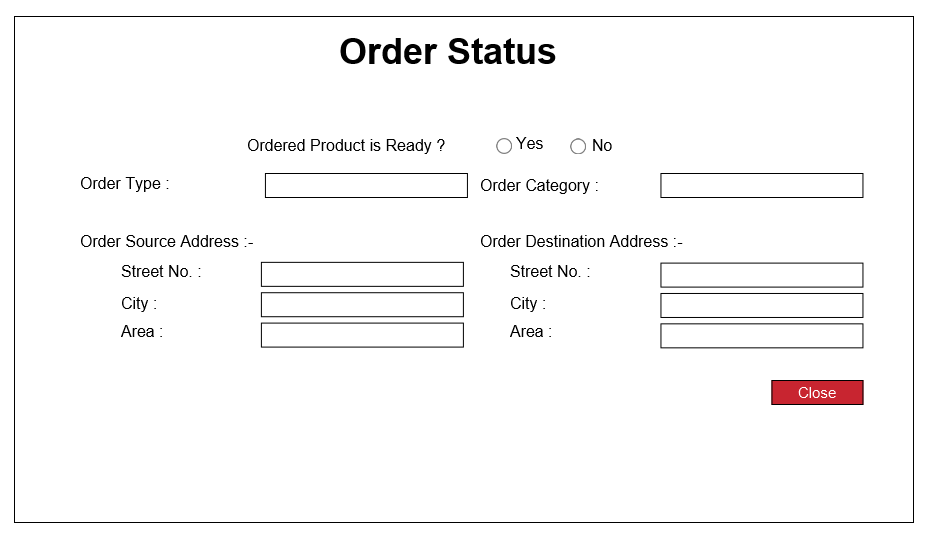
\includegraphics[scale=0.3]{./UIs for Latex Reports/UI-023 OrderStatus@1x.png}\end{center}  \\ \hline

Pre-Condition &  Order Details Form should open \\ \hline

Flow & Main Scenario:

\begin{enumerate}
\item   From Orders List Click on Check Status.
\item   A new Form Order Status will open
\end{enumerate}

\\ \hline
Post-Condition &  You can now track the progress of your order   \\ \hline

\end{tabular}
%------------------------------------------
\section{Use Case 17(Route Finder)}

\begin{tabular}{ | m{3cm} | m{12cm}| } \hline

Use Case ID &  U17 \\\hline

Name  	    & Route Finder  \\ \hline

Actor     	& Rider \\ \hline

Description & After the successful acceptance of certain order from warehouse, now rider has to select the best and the shortest path or route to the destination so his miscellaneous expenses (e.g., fuel) should be less. This allows him to select the shortest route. But he has been shown all possible routes.   \\ \hline

UI Interface in JUSTINMIND & \begin{center} 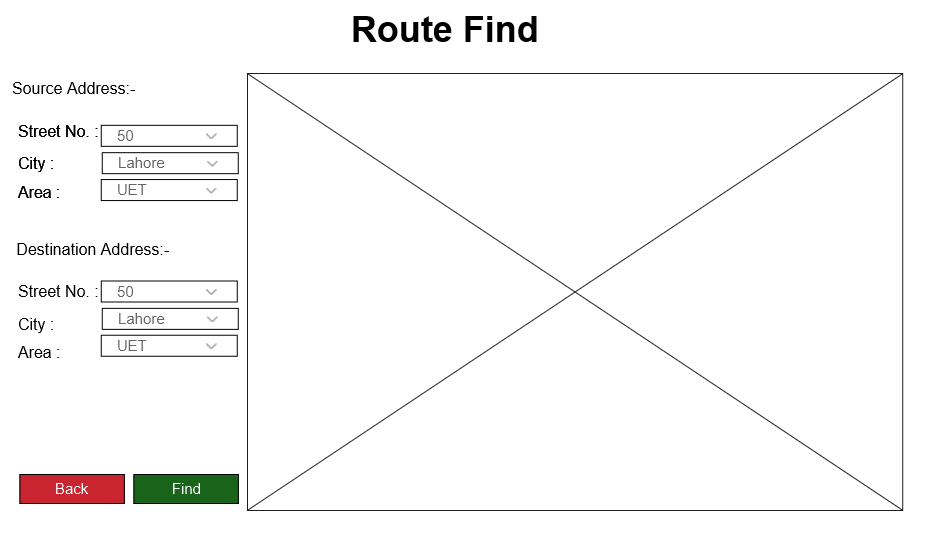
\includegraphics[scale=0.3]{./UIs for Latex Reports/UI-024 Route Finder@1x.png}\end{center}  \\ \hline

Pre-Condition &  Select Find Route from Rider’s Dashboard \\ \hline

Flow & Main Scenario:

\begin{enumerate}
\item   Route Find Form will open
\item   Fill Source Address
\item   Fill Destination Address
\item   Select Find


\end{enumerate}
\\ \hline
Post-Condition &  You will be shown all the possible routes from source to destination   \\ \hline

\end{tabular}
%------------------------------------------
\section{Use Case 18(Add Shopkeeper)}

\begin{tabular}{ | m{3cm} | m{12cm}| } \hline

Use Case ID & U18  \\\hline

Name  	    &  Add Shopkeeper \\ \hline

Actor     	& Rider, CEO, Employee \\ \hline

Description & Rider will approach the shopkeeper. If shopkeeper is not registered with the system before, the rider will register him first if the shopkeeper orders something. Second scenario may be the CEO and Employee both have the authority to add shopkeeper details what the rider would give them   \\ \hline

UI Interface in JUSTINMIND & \begin{center} 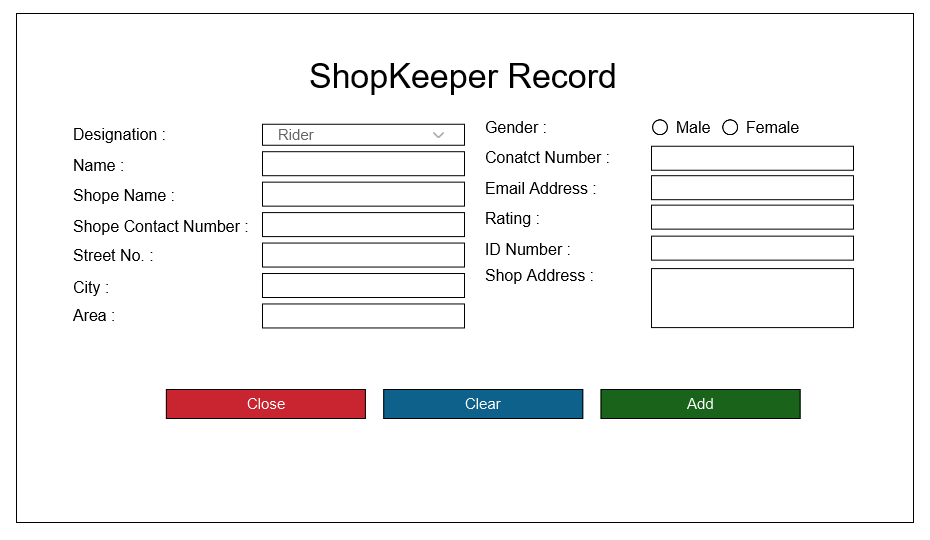
\includegraphics[scale=0.3]{./UIs for Latex Reports/UI-025 Add ShopKeeper@1x.png}\end{center}  \\ \hline

Pre-Condition & Select Add Shopkeeper from CEO’s, Rider’s, or Employee’s Dashboard  \\ \hline


Flow & Main Scenario:

\begin{enumerate}
\item   Select Appropriate Designation
\item  Fill all necessary details with the shop details as well
\item  Click Add button


\end{enumerate}

Alternate Flow:

\begin{itemize}
\item Clicking Clear Button
	\begin{enumerate}
		\item Will clear all the fields you have filled
	\end{enumerate}
\item 	Clicking Close Button
	\begin{enumerate}
	   	 \item	Will happen to return to the respective/corresponding dashboard
	\end{enumerate}
\item If all necessary field are not filled
	\begin{enumerate}
		\item Alert Message will occur
		\item Control will remain on the same page
	\end{enumerate}
\end{itemize}
\\ \hline
Post-Condition &  Shopkeeper Information will be added to your system   \\ \hline

\end{tabular}
%------------------------------------------
\section{Use Case 19(Add Payment) }

\begin{tabular}{ | m{3cm} | m{12cm}| } \hline

Use Case ID &  U19 \\\hline

Name  	    & Add  Payment  \\ \hline

Actor     	& Rider, Employee, CEO \\ \hline

Description & Rider will approach the shopkeeper. Took Payment from the shopkeeper and add it into the system. \\ \hline

UI Interface in JUSTINMIND & \begin{center} 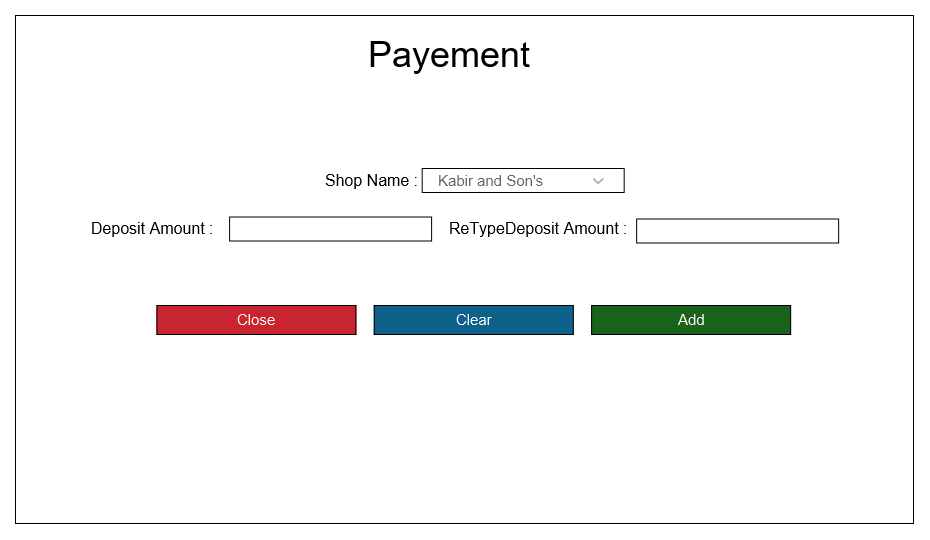
\includegraphics[scale=0.3]{./UIs for Latex Reports/UI-026 Add Payment@1x.png}\end{center}  \\ \hline

Pre-Condition &  Select Add Payment from Rider’s Dashboard(Shopkeeper Must be registered first) \\ \hline

\end{tabular} \newpage \begin{tabular}{ | m{3cm} | m{12cm}| }  \hline
Flow & Main Scenario:

\begin{enumerate}
\item   Payment Form will open
\item   Select Shop Name (it should be registered first)
\item   Add Deposit Amount and Confirm
\item   Click Add


\end{enumerate}

Alternate Flow:

\begin{itemize}
\item 	Clicking Clear Button
	\begin{enumerate}
		\item Will clear all the fields you have filled
	\end{enumerate}
\item Clicking Close Button
	\begin{enumerate}
	   	 \item	Will happen to return to the respective/corresponding dashboard
	\end{enumerate}
\item If deposit amount and Retype Deposit Amount are not same
	\begin{enumerate}
		\item Error Message will occur
		\item System will return to the same page after clicking on OK button
	\end{enumerate}
\end{itemize}
\\ \hline
Post-Condition &   Payment will be accepted for the selected shopkeeper  \\ \hline

\end{tabular}
%------------------------------------------
\section{Use Case 20(Withdraw Expenses) }

\begin{tabular}{ | m{3cm} | m{12cm}| } \hline

Use Case ID & U20  \\\hline

Name  	    &  Withdraw Expenses \\ \hline

Actor     	&  CEO \\ \hline

Description & --- \\ \hline

UI Interface in JUSTINMIND & \begin{center} 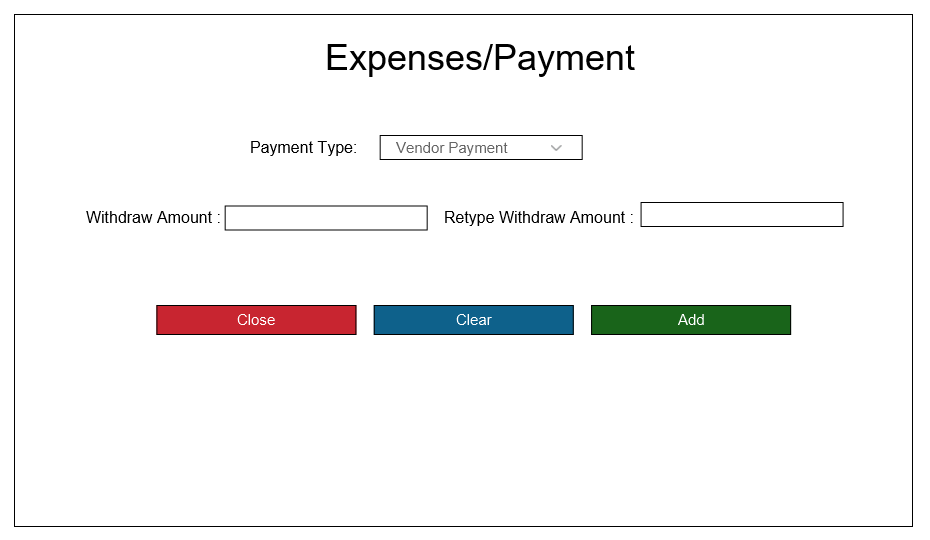
\includegraphics[scale=0.3]{./UIs for Latex Reports/UI-027 Add Withdraw Expenses@1x.png}\end{center}  \\ \hline

Pre-Condition &   \\ \hline

\end{tabular} \newpage \begin{tabular}{ | m{3cm} | m{12cm}| }  \hline
Flow & Main Scenario:

\begin{enumerate}
\item   Payment Form will open
\item Select Payment Type
\item Type Withdraw Amount and Retype it in the next box
\item Click Add


\end{enumerate}

Alternate Flow:

\begin{itemize}
\item Clicking Clear Button
	\begin{enumerate}
		\item Will clear all the fields you have filled
	\end{enumerate}
\item Clicking Close Button
	\begin{enumerate}
	   	 \item	Will happen to return to the respective/corresponding dashboard
	\end{enumerate}
\item If Withdraw amount and Retype Withdraw Amount are not same
	\begin{enumerate}
		\item Error Message will occur
		\item System will return to the same page after clicking on OK button
	\end{enumerate}
\end{itemize}
\\ \hline
Post-Condition &    \\ \hline

\end{tabular}
%------------------------------------------

\section{Use Case 21(Create Account)}

\begin{tabular}{ | m{3cm} | m{12cm}| } \hline

Use Case ID &  U21 \\\hline

Name  	    & Create Account  \\ \hline

Actor     	& All \\ \hline

Description & All actors can link with the system by creating account and register themselves for this system. Provide Necessary Information and you can dive into the system by logging into the system. \\ \hline

UI Interface in JUSTINMIND & \begin{center} 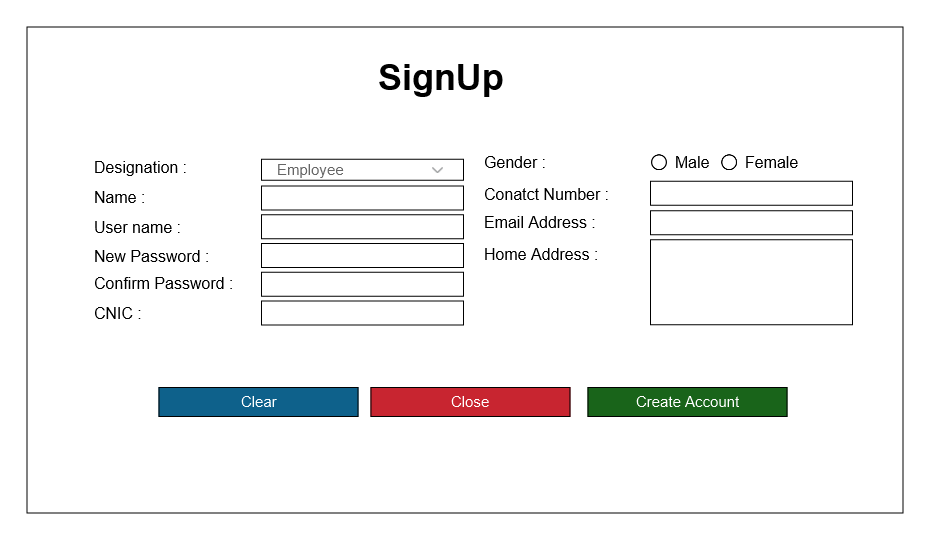
\includegraphics[scale=0.3]{./UIs for Latex Reports/UI-004 Create Account@1x.png}\end{center}  \\ \hline

Pre-Condition &  System Will Initiate with this page \\ \hline


Flow & Main Scenario:

\begin{enumerate}
\item   Select Your Designation
\item  Provide All Necessary Details
\item  Click on Create Account


\end{enumerate}

\\ \hline
Post-Condition &  You are now the user of this system  \\ \hline

\end{tabular}
%------------------------------------------
\newpage
\chapter {Use Interfaces}
\section{Intro}

\begin{tabular}{ | m{3cm} | m{12cm}| } \hline

Interface ID & I01  \\\hline

Name  	      & Intro  \\ \hline

Linked Use Case & NULL \\ \hline

UI Interface in JUSTINMIND & \begin{center} 
\includegraphics[scale=0.3]{./UIs for Latex Reports/UI-001 Intro@1x.png}\end{center}  \\ \hline
\end{tabular} 
%------------------------------------------
\section{Login}

\begin{tabular}{ | m{3cm} | m{12cm}| } \hline

Interface ID & I02  \\\hline

Name  	      & Login  \\ \hline

Linked Use Case & U01 \\ \hline

UI Interface in JUSTINMIND & \begin{center} 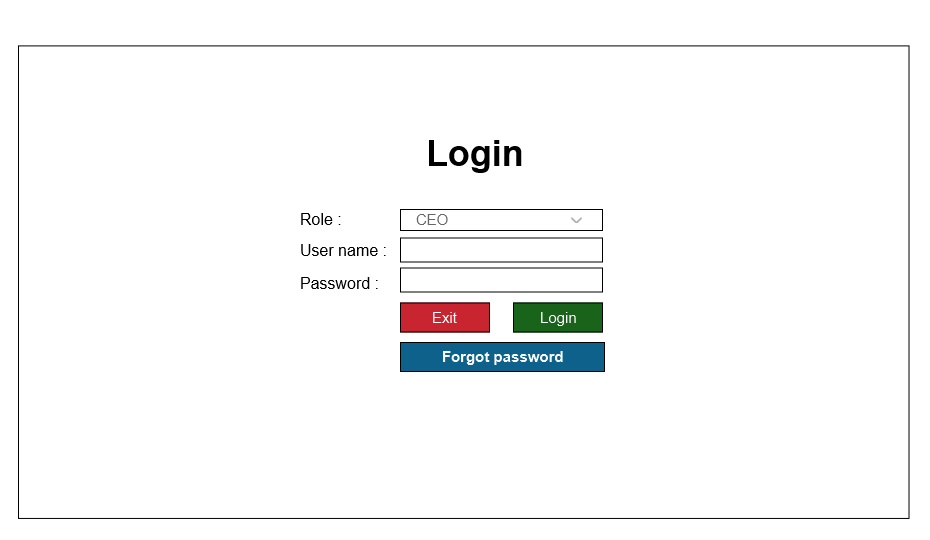
\includegraphics[scale=0.3]{./UIs for Latex Reports/UI-002 Login@1x.png}\end{center}  \\ \hline

Validators & 
\begin{itemize}
\item   Password Validations (Must be of 8 characters)
\item   User Validation(Check if user exist or not)

\end{itemize}
\\ \hline

\end{tabular} 
%------------------------------------------
\section{Forgot Password }

\begin{tabular}{ | m{3cm} | m{12cm}| } \hline

Interface ID &  103 \\\hline

Name  	      & Forgot Password  \\ \hline

Linked Use Case &  \\ \hline

UI Interface in JUSTINMIND & \begin{center} 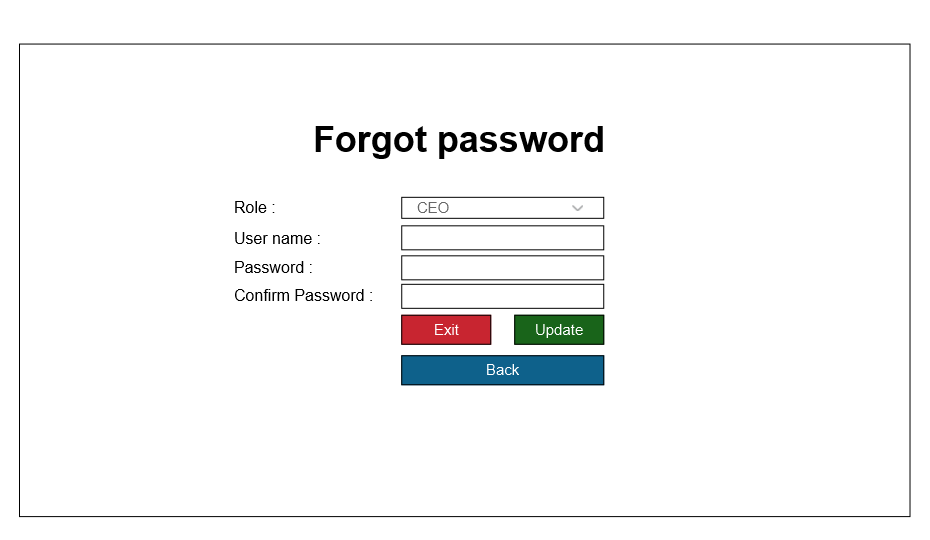
\includegraphics[scale=0.3]{./UIs for Latex Reports/UI-003 Forgot password@1x.png}\end{center}  \\ \hline

Validators & 
\begin{itemize}
\item  New Password must be different from previous password
\item  Username Validation
\item  Password and Confirm Password Textbox are Same or not
\end{itemize}
\\ \hline

\end{tabular} 
%------------------------------------------
\section{Create Account }

\begin{tabular}{ | m{3cm} | m{12cm}| } \hline

Interface ID &   104 \\\hline

Name  	      &   Create Account\\ \hline

Linked Use Case &  U21\\ \hline

UI Interface in JUSTINMIND & \begin{center} 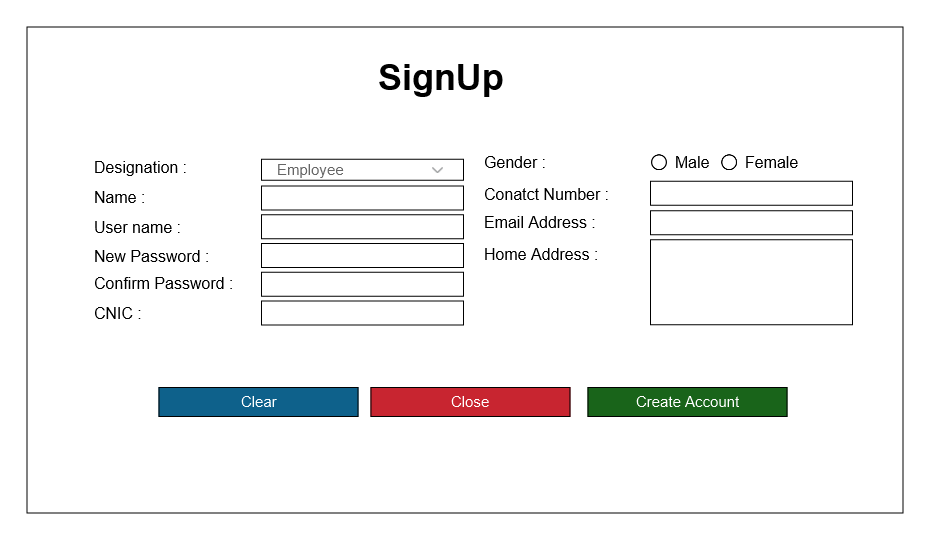
\includegraphics[scale=0.3]{./UIs for Latex Reports/UI-004 Create Account@1x.png}\end{center}  \\ \hline

Validators & 
\begin{itemize}
\item   New Password and Confirmation password must be the same
\item  CNIC must be of 13 digits
\item  Contact Number must be of 11 digits
\item  All Information must be provided before account creation
\item  Email Validations


\end{itemize}
\\ \hline

\end{tabular} 
%------------------------------------------

\section{Update Information}

\begin{tabular}{ | m{3cm} | m{12cm}| } \hline

Interface ID &  I05 \\\hline

Name  	      &  Update Information \\ \hline

Linked Use Case &  \\ \hline

UI Interface in JUSTINMIND & \begin{center} 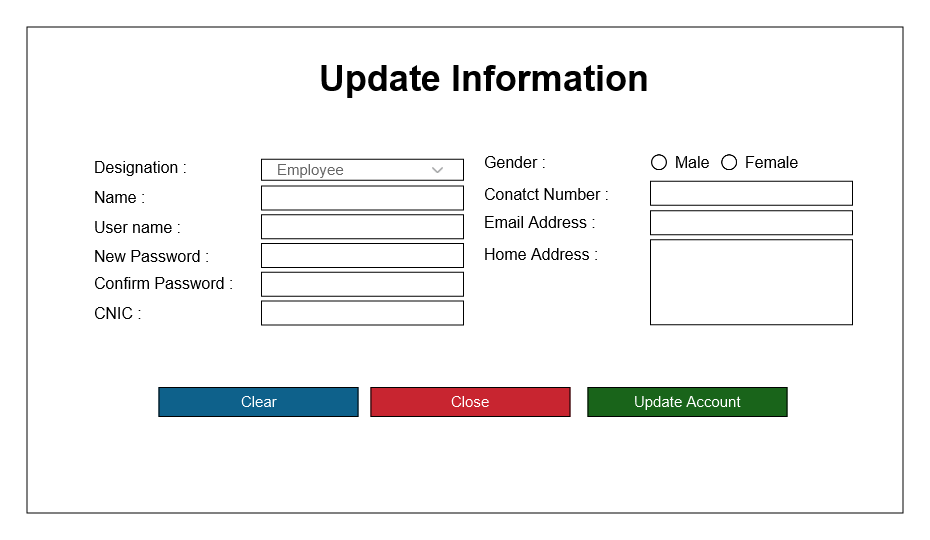
\includegraphics[scale=0.3]{./UIs for Latex Reports/UI-005 Update Account@1x.png}\end{center}  \\ \hline

Validators & 
\begin{itemize}
\item   New Password and Confirmation password must be the same
\item CNIC must be of 13 digits
\item Contact Number must be of 11 digits
\item All Information must be provided before account creation
\item Email Validations


\end{itemize}
\\ \hline

\end{tabular} 
%------------------------------------------
\section{Account Detail }

\begin{tabular}{ | m{3cm} | m{12cm}| } \hline

Interface ID &  I06 \\\hline

Name  	      &  Account Detail \\ \hline

Linked Use Case & U04 \\ \hline

UI Interface in JUSTINMIND & \begin{center} 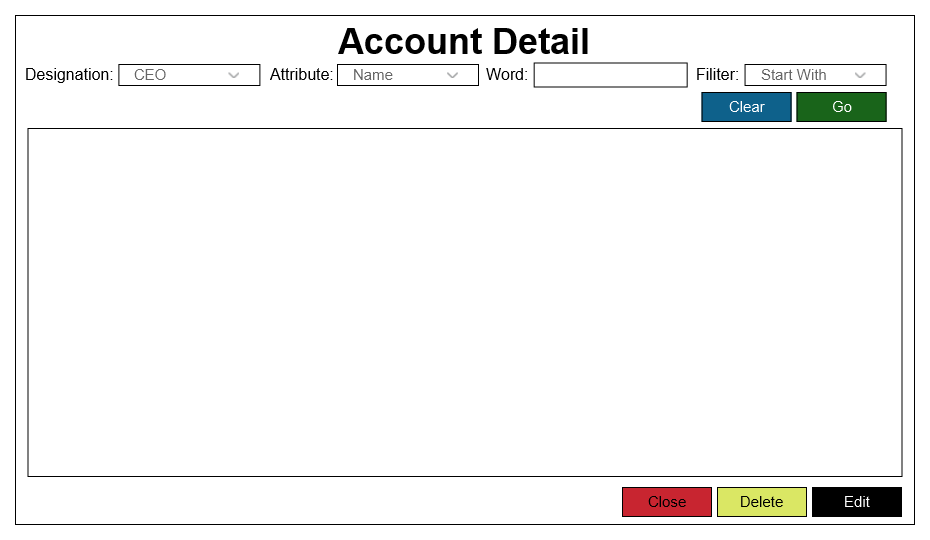
\includegraphics[scale=0.3]{./UIs for Latex Reports/UI-006 ViewsAndDelete Account@1x.png}\end{center}  \\ \hline

Validators & 
\begin{itemize}
\item   On clicked delete and edit button there is must to select any column first from grid list. 
\item  Filters must be applied before clicking Go


\end{itemize}
\\ \hline

\end{tabular} 
%------------------------------------------
\section{CEO Dashboard }

\begin{tabular}{ | m{3cm} | m{12cm}| } \hline

Interface ID &  I07 \\\hline

Name  	      & CEO Dashboard  \\ \hline

Linked Use Case & U03 \\ \hline

UI Interface in JUSTINMIND & \begin{center} 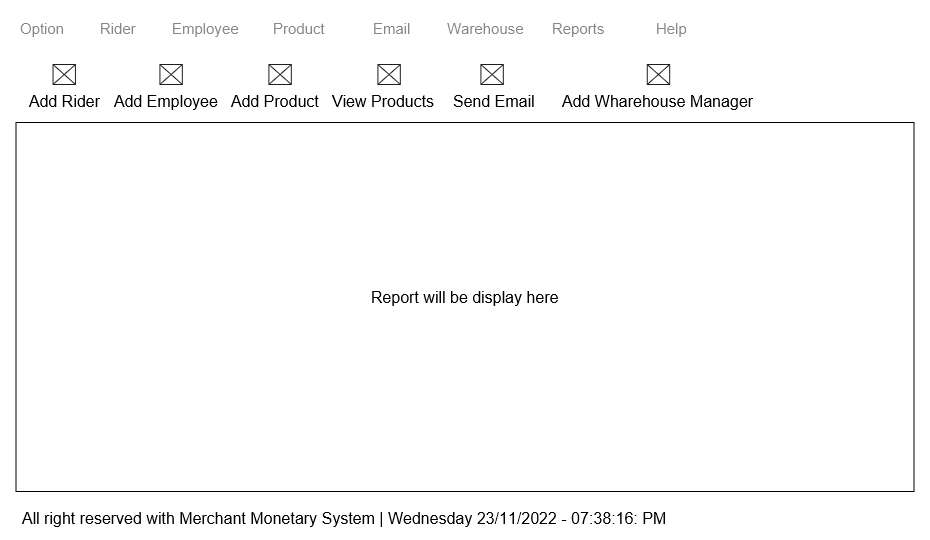
\includegraphics[scale=0.3]{./UIs for Latex Reports/UI-007 CEO Dashboard@1x.png}\end{center}  \\ \hline

\end{tabular} 
%------------------------------------------
\section{Add Product }

\begin{tabular}{ | m{3cm} | m{12cm}| } \hline

Interface ID & I08  \\\hline

Name & Add Product  \\ \hline

Linked Use Case & U06	 \\ \hline

UI Interface in JUSTINMIND & \begin{center} 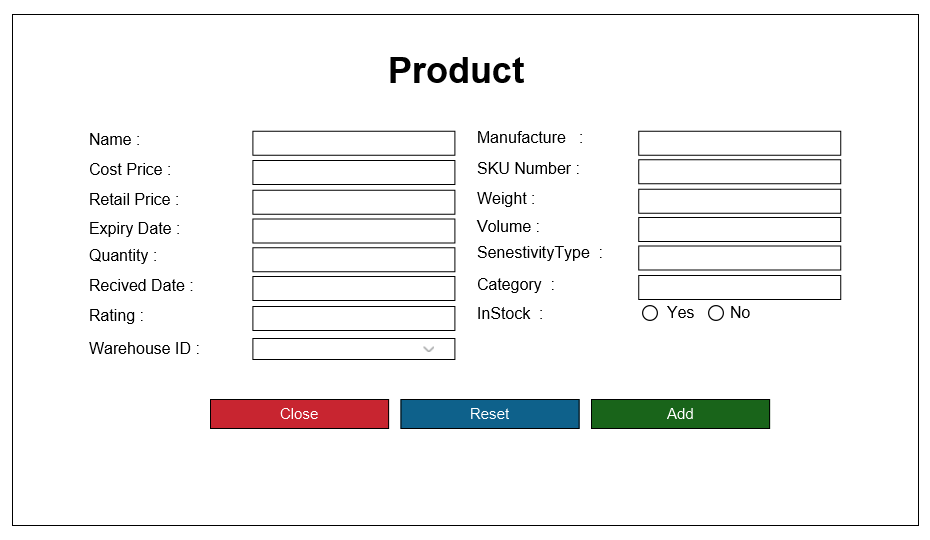
\includegraphics[scale=0.3]{./UIs for Latex Reports/UI-008 Add Product@1x.png}\end{center}  \\ \hline

Validators & 
\begin{itemize}
\item   Product Name must contain only Digits and alphabets.
\item Cost Price must not be negative.
\item The date must be positive. And not previous than current.
\item Quantity must be positive. And not in decimals.
\item Rating must be positive and integer.
\item SKU-ID must be positive.
\item Weight and Volume must be in integers and decimals and positive.
\item IN Stock check box must be filled.


\end{itemize}
\\ \hline

\end{tabular} 
%------------------------------------------
\section{Update Product }

\begin{tabular}{ | m{3cm} | m{12cm}| } \hline

Interface ID & I09  \\\hline

Name  &  Update Product \\ \hline

Linked Use Case & U08	  \\ \hline

UI Interface in JUSTINMIND & \begin{center} 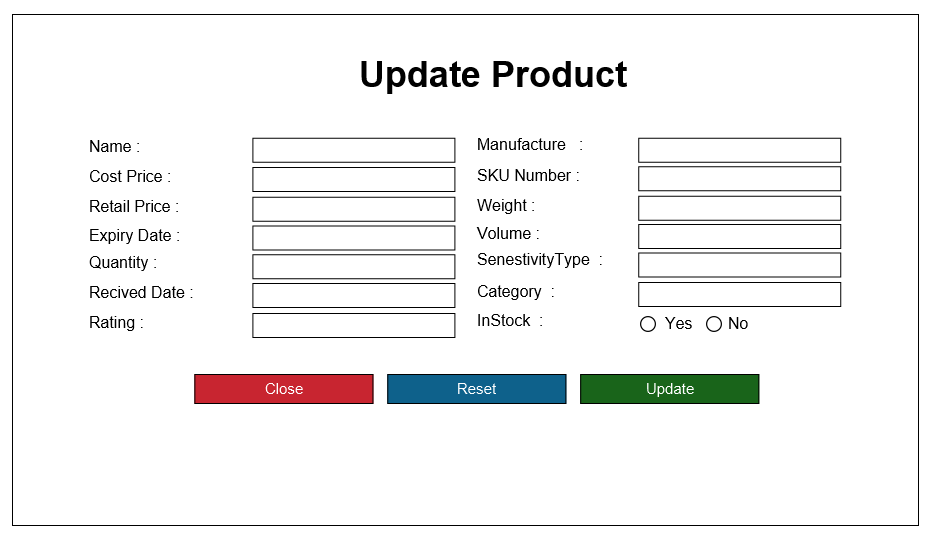
\includegraphics[scale=0.3]{./UIs for Latex Reports/UI-009 Update Product@1x.png}\end{center}  \\ \hline

Validators & 
\begin{itemize}
\item   Product Name must contain only Digits and alphabets.
\item Cost Price must not be negative.
\item The date must be positive. And not previous than current.
\item Quantity must be positive. And not in decimals.
\item Rating must be positive and integer.
\item SKU-ID must be positive.
\item Weight and Volume must be in integers and decimals and positive.
\item IN Stock check box must be filled.


\end{itemize}
\\ \hline

\end{tabular} 
%------------------------------------------
\section{Product Detail }

\begin{tabular}{ | m{3cm} | m{12cm}| } \hline

Interface ID &  I10 \\\hline

Name  &  Product Detail \\ \hline

Linked Use Case & U07	 \\ \hline

UI Interface in JUSTINMIND & \begin{center} 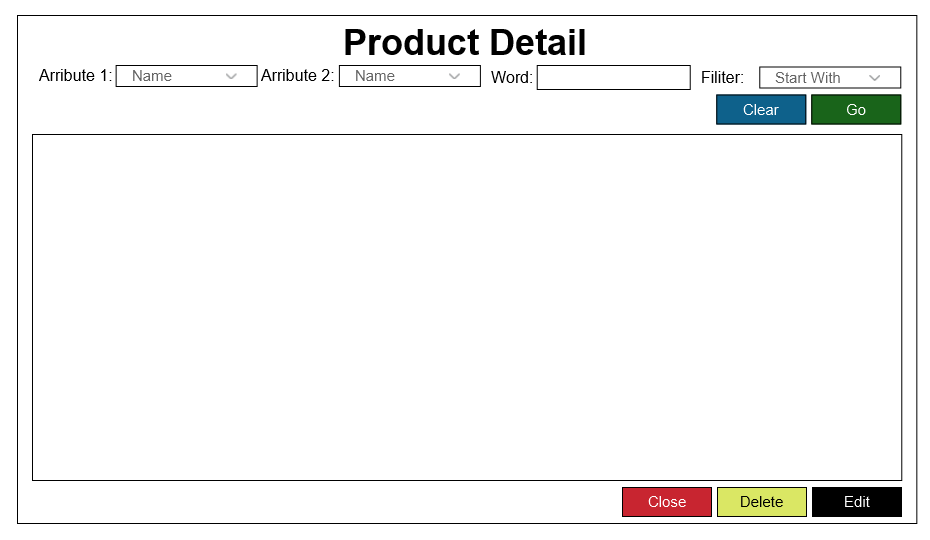
\includegraphics[scale=0.3]{./UIs for Latex Reports/UI-010 ViewAndDelete Products@1x.png}\end{center}  \\ \hline

Validators & 
\begin{itemize}
\item   On clicked delete and edit button there is must to select any column first from grid list. 
\item  Filters must be applied before clicking Go.


\end{itemize}
\\ \hline

\end{tabular} 
%------------------------------------------
\section{Order Product}

\begin{tabular}{ | m{3cm} | m{12cm}| } \hline

Interface ID & I11  \\\hline

Name  &  Order Product \\ \hline

Linked Use Case & U11	 \\ \hline

UI Interface in JUSTINMIND & \begin{center} 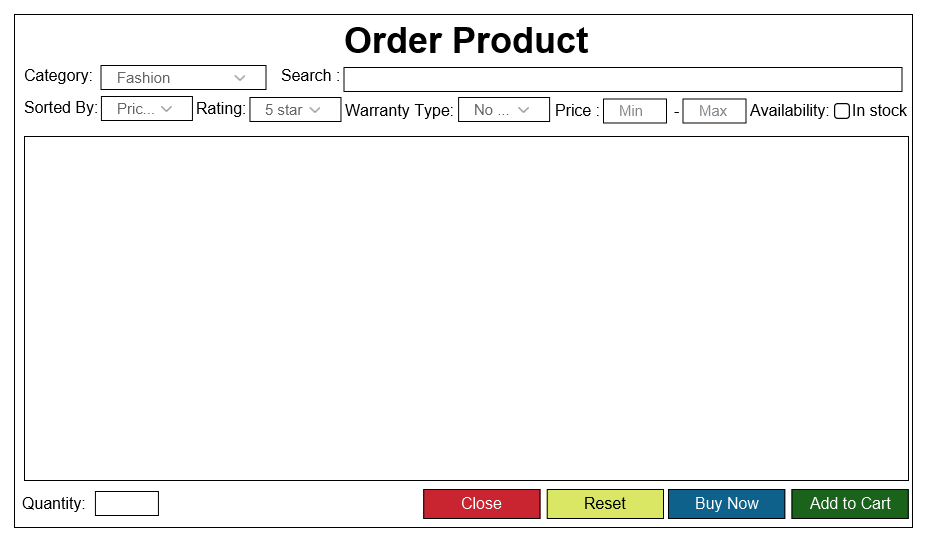
\includegraphics[scale=0.3]{./UIs for Latex Reports/UI-011 Order Product@1x.png}\end{center}  \\ \hline

Validators & 
\begin{itemize}
\item   
Price must be positive.
\item 
Search text only contains alphabets and integers only.

\end{itemize}
\\ \hline

\end{tabular} 
%------------------------------------------
\section{Order Summary}

\begin{tabular}{ | m{3cm} | m{12cm}| } \hline

Interface ID & I12  \\\hline

Name  & Order Summary  \\ \hline

Linked Use Case & U11 \\ \hline

UI Interface in JUSTINMIND & \begin{center} 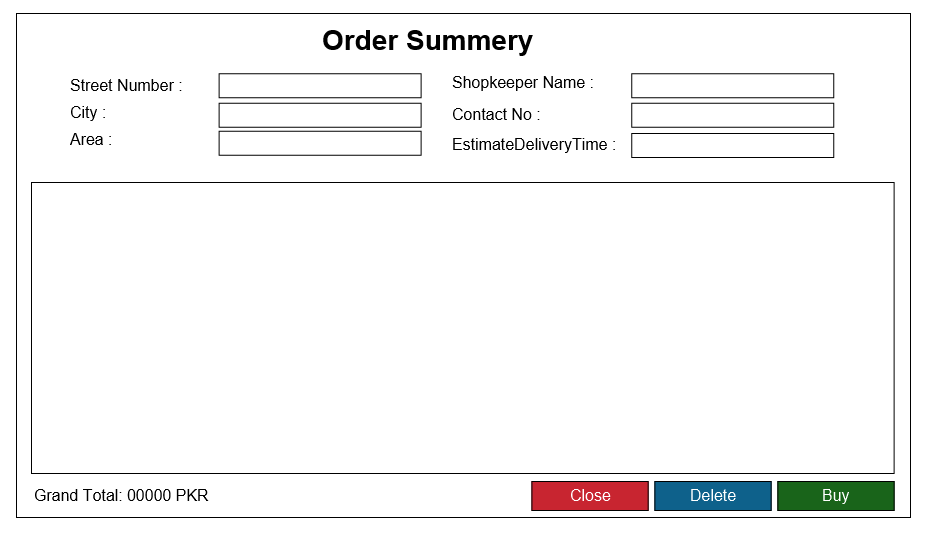
\includegraphics[scale=0.3]{./UIs for Latex Reports/UI-012 Order Summery@1x.png}\end{center}  \\ \hline

Validators & 
\begin{itemize}
\item   Street No. must be integer
\item   Contact No. must be of 11 digits
\item   Delivery time must be a number may be float or integer
\item   All fields must be typed before buying products


\end{itemize}
\\ \hline

\end{tabular} 
%------------------------------------------
\section{Send Email }

\begin{tabular}{ | m{3cm} | m{12cm}| } \hline

Interface ID & I13  \\\hline

Name  &  Send Email \\ \hline

Linked Use Case & U12 \\ \hline

UI Interface in JUSTINMIND & \begin{center} 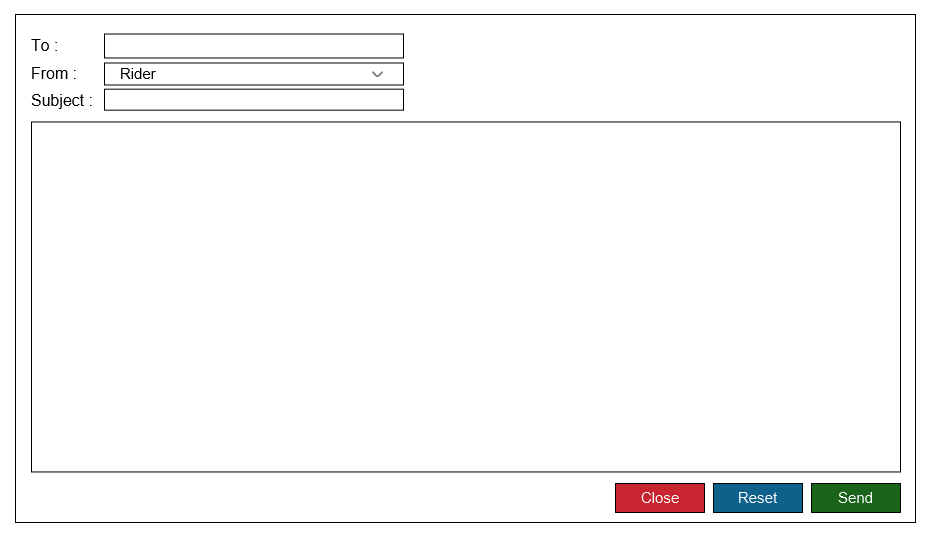
\includegraphics[scale=0.3]{./UIs for Latex Reports/UI-013 SendEmail@1x.png}\end{center}  \\ \hline

Validators & 
\begin{itemize}
\item  To section must be filled to send the mail.



\end{itemize}
\\ \hline

\end{tabular} 
%------------------------------------------
\section{New Warehouse}

\begin{tabular}{ | m{3cm} | m{12cm}| } \hline

Interface ID &  I14 \\\hline

Name  & New Warehouse  \\ \hline

Linked Use Case & U13	 \\ \hline

UI Interface in JUSTINMIND & \begin{center} 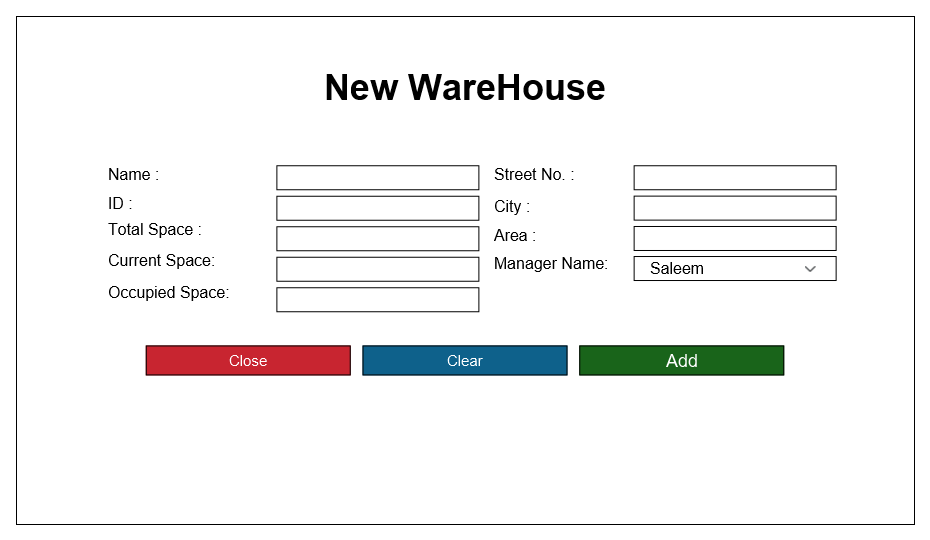
\includegraphics[scale=0.3]{./UIs for Latex Reports/UI-014 AddWarehouse@1x.png}\end{center}  \\ \hline

Validators & 
\begin{itemize}
\item   Space fields and Street No. input must be a number
\item  Necessary fields must be filled before updating


\end{itemize}
\\ \hline

\end{tabular} 
%------------------------------------------
\section{Update Warehouse }

\begin{tabular}{ | m{3cm} | m{12cm}| } \hline

Interface ID & I15  \\\hline

Name  &  Update Warehouse \\ \hline

Linked Use Case & U15 \\ \hline

UI Interface in JUSTINMIND & \begin{center} 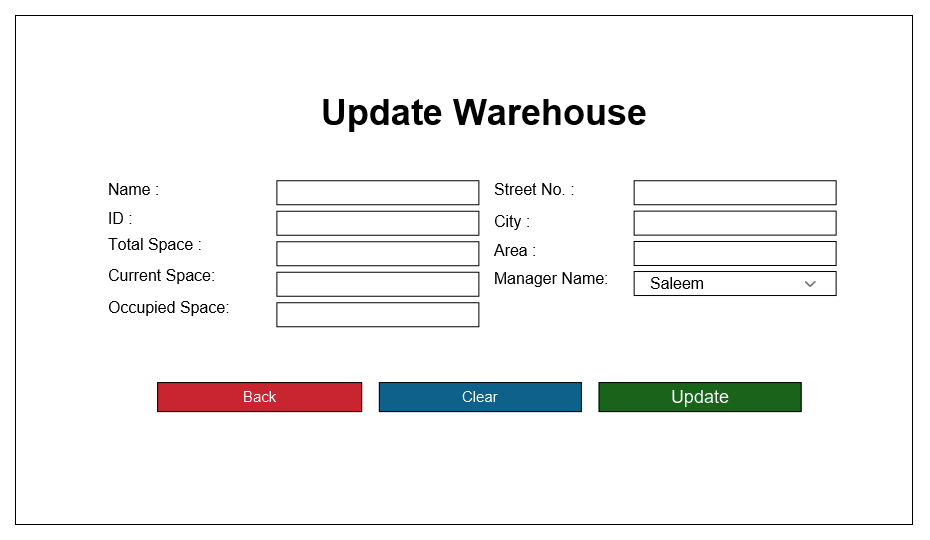
\includegraphics[scale=0.3]{./UIs for Latex Reports/UI-015 EditWarehouse@1x.png}\end{center}  \\ \hline

Validators & 
\begin{itemize}
\item   Space fields and Street No. input must be a number
\item  Necessary fields must be filled before updating


\end{itemize}
\\ \hline

\end{tabular} 
%------------------------------------------
\section{Warehouse Detail }

\begin{tabular}{ | m{3cm} | m{12cm}| } \hline

Interface ID & I16  \\\hline

Name  &  Warehouse Detail \\ \hline

Linked Use Case & U14 \\ \hline

UI Interface in JUSTINMIND & \begin{center} 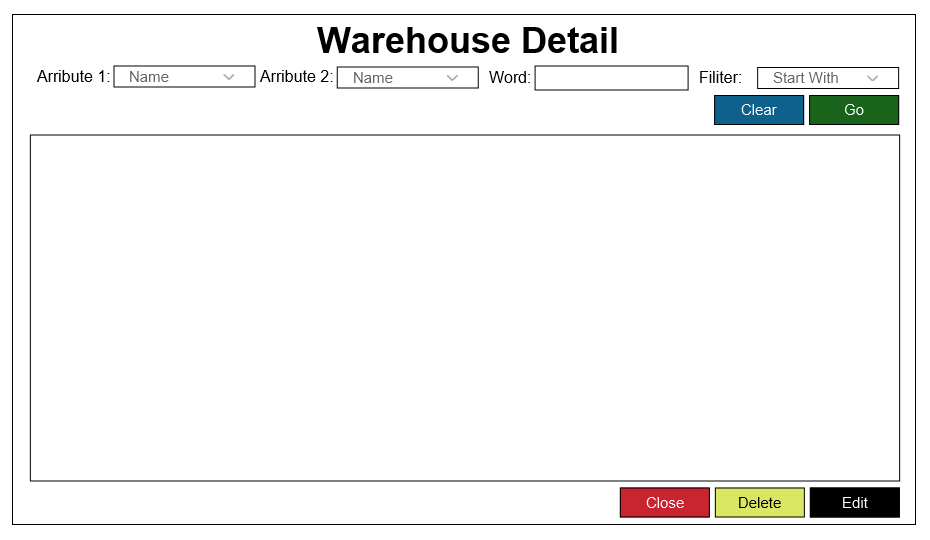
\includegraphics[scale=0.3]{./UIs for Latex Reports/UI-016 ViewAndDelete Warehouse@1x.png}\end{center}  \\ \hline

Validators & 
\begin{itemize}
\item   On clicked delete and edit button there is must to select any row first from grid list. 
\item  Filters must be applied before clicking Go


\end{itemize}
\\ \hline

\end{tabular} 
%------------------------------------------
\section{Warehouse Manager Dashboard }

\begin{tabular}{ | m{3cm} | m{12cm}| } \hline

Interface ID &  I17 \\\hline

Name  &  Warehouse Manager Dashboard \\ \hline

Linked Use Case & NILL \\ \hline

UI Interface in JUSTINMIND & \begin{center} 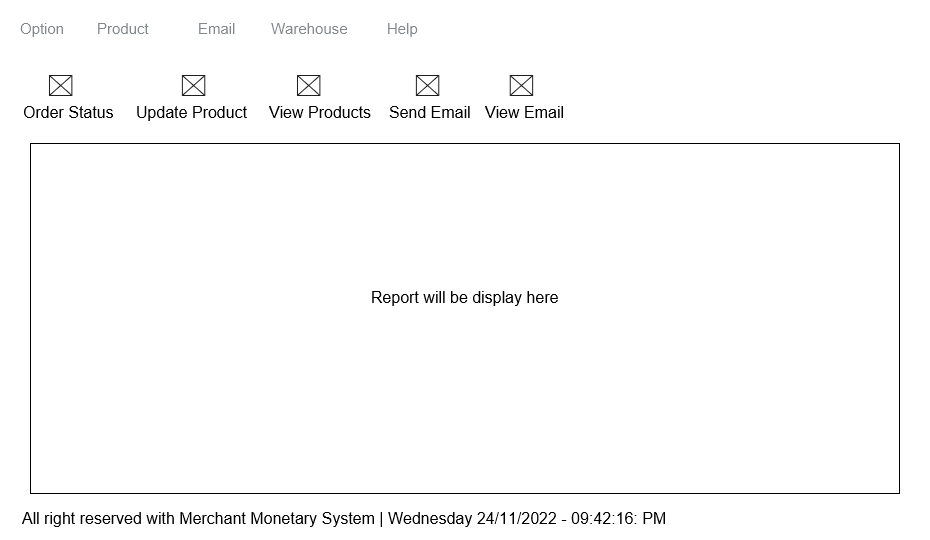
\includegraphics[scale=0.3]{./UIs for Latex Reports/UI-017 Warehouse Manager Dashboard@1x.png}\end{center}  \\ \hline


\end{tabular} 
%------------------------------------------
\section{Employee Dashboard }

\begin{tabular}{ | m{3cm} | m{12cm}| } \hline

Interface ID & I18  \\\hline

Name  &  Employee Dashboard \\ \hline

Linked Use Case &  NILL \\ \hline

UI Interface in JUSTINMIND & \begin{center} 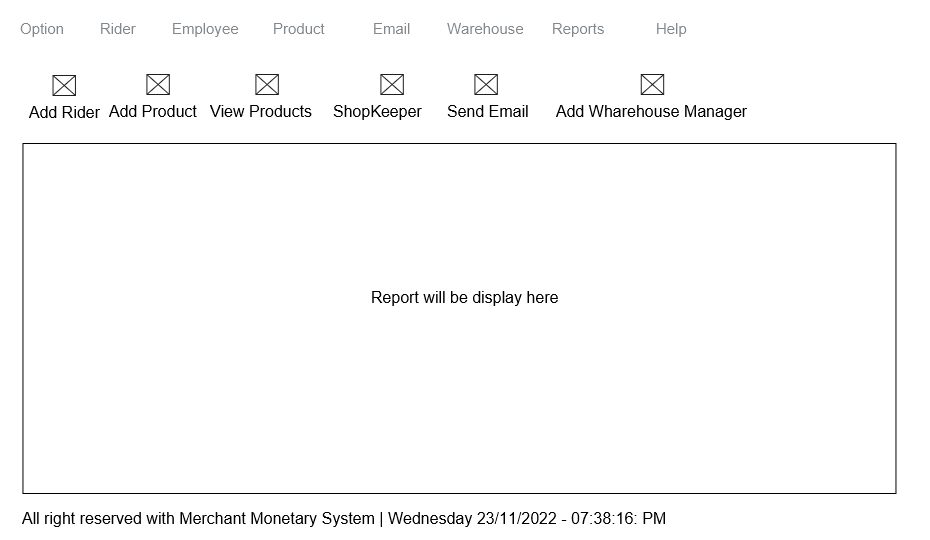
\includegraphics[scale=0.3]{./UIs for Latex Reports/UI-018 Employee Dashboard@1x.png}\end{center}  \\ \hline

\end{tabular} 
%------------------------------------------
\section{Rider Dashboard }

\begin{tabular}{ | m{3cm} | m{12cm}| } \hline

Interface ID & I19  \\\hline

Name  & Rider Dashboard  \\ \hline

Linked Use Case & NILL  \\ \hline

UI Interface in JUSTINMIND & \begin{center} 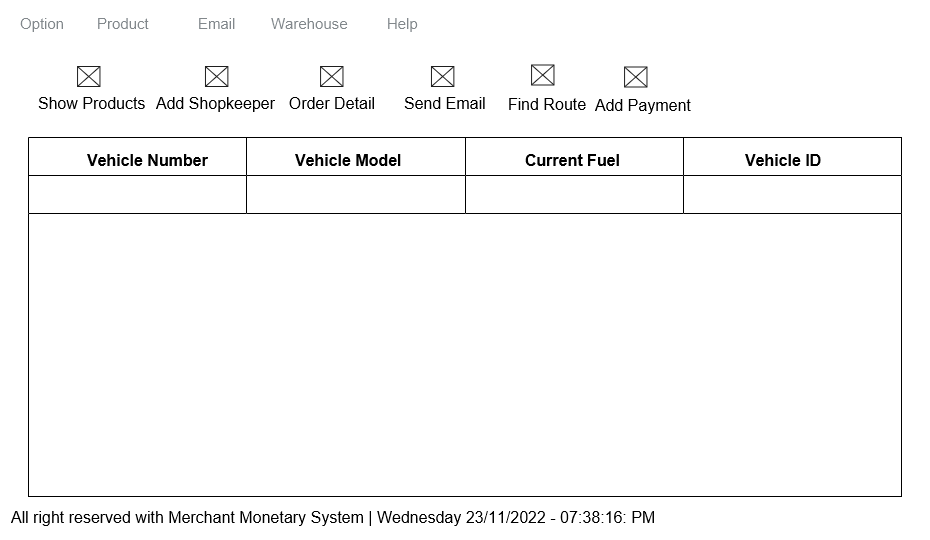
\includegraphics[scale=0.3]{./UIs for Latex Reports/UI-019 Rider Dashboard@1x.png}\end{center}  \\ \hline

\end{tabular} 
%------------------------------------------
\section{Add Rider }

\begin{tabular}{ | m{3cm} | m{12cm}| } \hline

Interface ID & I20  \\\hline

Name  &   \\ \hline

Linked Use Case & U09 \\ \hline

UI Interface in JUSTINMIND & \begin{center} 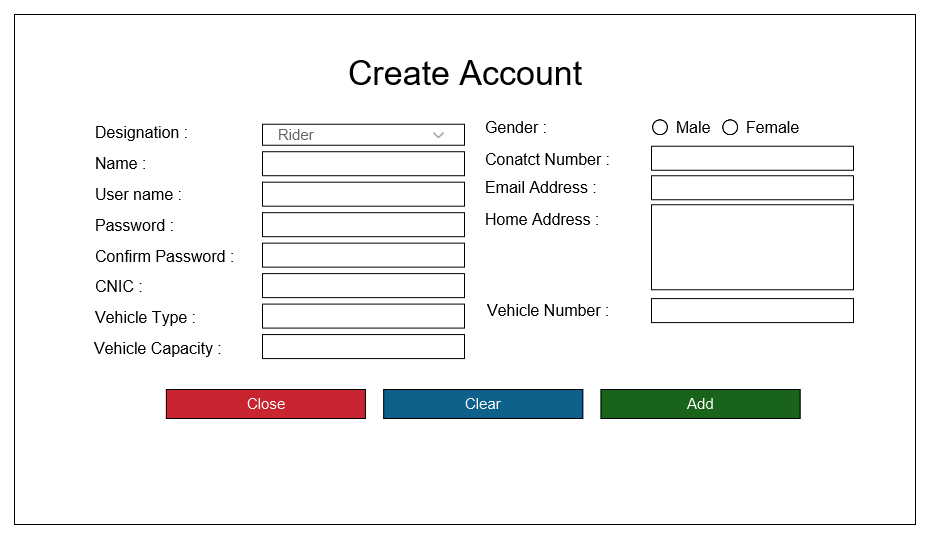
\includegraphics[scale=0.3]{./UIs for Latex Reports/UI-020 AddRider@1x.png}\end{center}  \\ \hline

Validators & 
\begin{itemize}
\item   Name Text Box must contain only alphabets.
\item The new Password and confirmation password
\item CNIC number must be of 13 digits.
\item Contact number must be of 11 digits.
\item Any text box value will not be added as negative.
\item All fields must be filled
\item Email validation


\end{itemize}
\\ \hline

\end{tabular} 
%------------------------------------------
\section{Update Rider }

\begin{tabular}{ | m{3cm} | m{12cm}| } \hline

Interface ID &  I21 \\\hline

Name  &  Update Rider \\ \hline

Linked Use Case & U10 \\ \hline

UI Interface in JUSTINMIND & \begin{center} 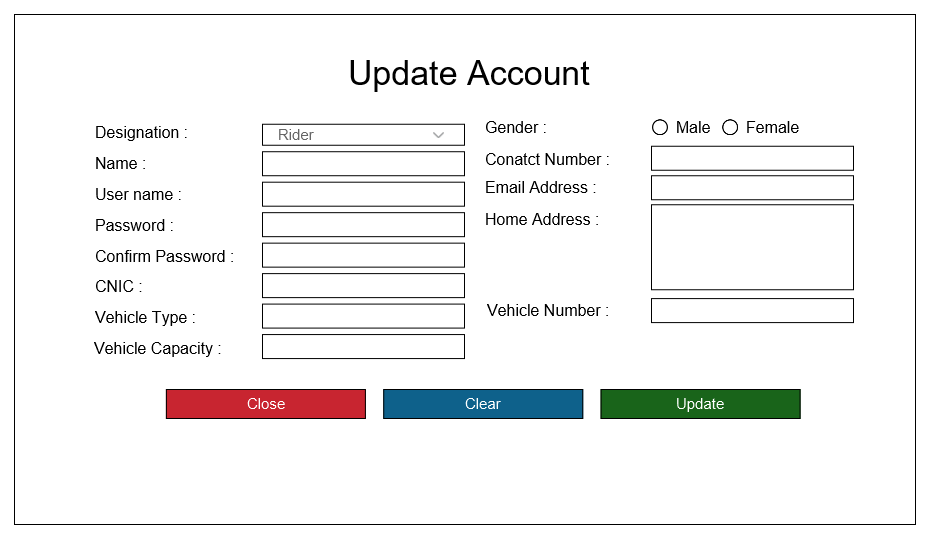
\includegraphics[scale=0.3]{./UIs for Latex Reports/UI-021 UpdateRider@1x.png}\end{center}  \\ \hline

Validators & 
\begin{itemize}
\item   Name Text Box must contain only alphabets.
\item  New Password must be different form last password
\item  The new Password and confirmation password
\item  CNIC number must be of 13 digits.
\item  Contact number must be of 11 digits.
\item  Any text box value will not be added as negative.
\item  All fields must be filled
\item  Email validation


\end{itemize}
\\ \hline

\end{tabular} 
%------------------------------------------
\section{Order Status }

\begin{tabular}{ | m{3cm} | m{12cm}| } \hline

Interface ID & I22  \\\hline

Name  & Order Status  \\ \hline

Linked Use Case &U16  \\ \hline

UI Interface in JUSTINMIND & \begin{center} 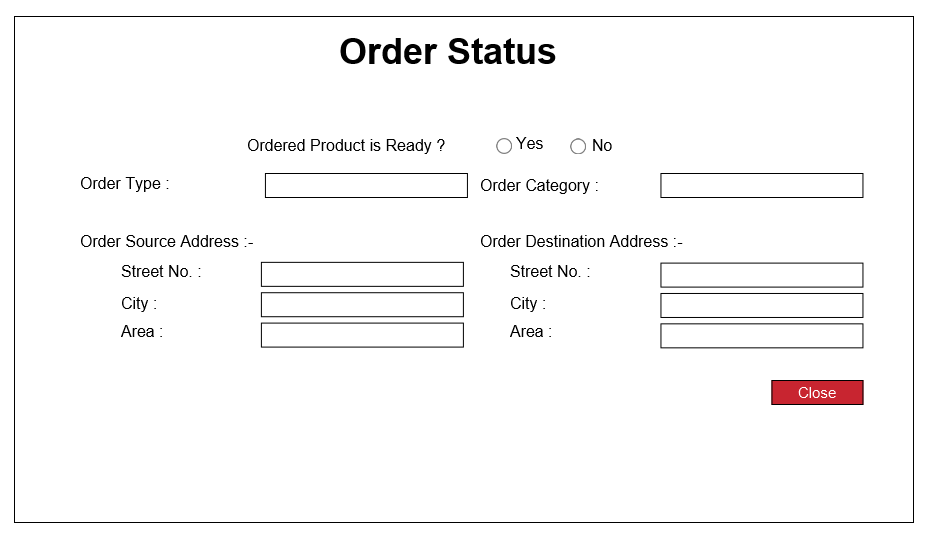
\includegraphics[scale=0.3]{./UIs for Latex Reports/UI-023 OrderStatus@1x.png}\end{center}  \\ \hline

\end{tabular} 
%------------------------------------------
\section{Order Status }

\begin{tabular}{ | m{3cm} | m{12cm}| } \hline

Interface ID &  I23 \\\hline

Name  & Order Status  \\ \hline

Linked Use Case & U17 \\ \hline

UI Interface in JUSTINMIND & \begin{center} 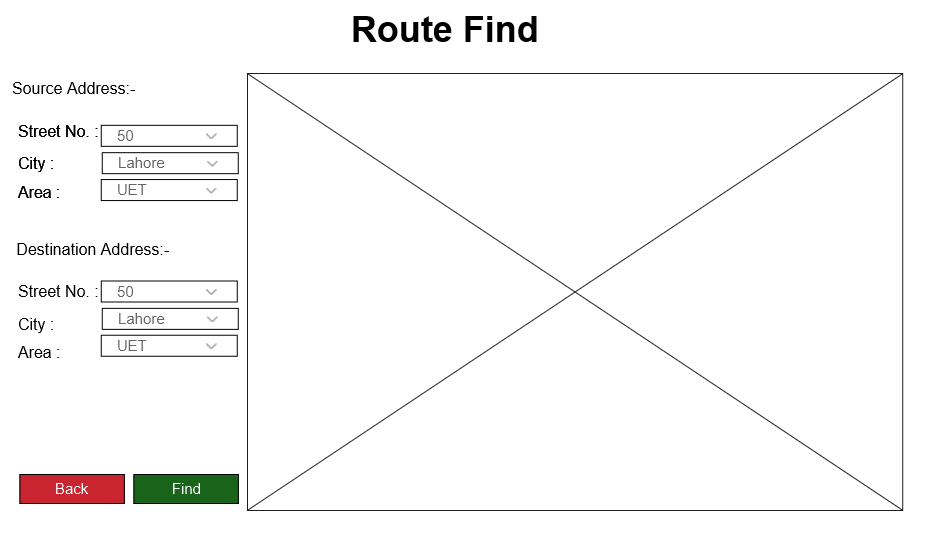
\includegraphics[scale=0.3]{./UIs for Latex Reports/UI-024 Route Finder@1x.png}\end{center}  \\ \hline

Validators & 
\begin{itemize}
\item  Street No. Must not be negative
\item All fields must be appropriately filled to find the routes
 

\end{itemize}
\\ \hline

\end{tabular} 
%------------------------------------------
\section{Shopkeeper Record }

\begin{tabular}{ | m{3cm} | m{12cm}| } \hline

Interface ID &  I24 \\\hline

Name  & Shopkeeper Record  \\ \hline

Linked Use Case & U18 \\ \hline

UI Interface in JUSTINMIND & \begin{center} 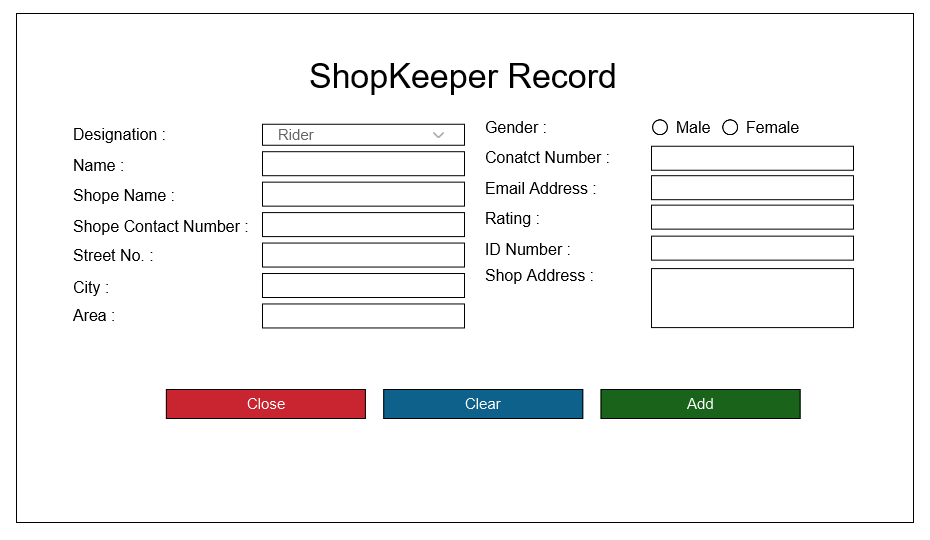
\includegraphics[scale=0.3]{./UIs for Latex Reports/UI-025 Add ShopKeeper@1x.png}\end{center}  \\ \hline

Validators & 
\begin{itemize}
\item  Email Validation
\item Contact Number Validation
\item Street No. must be a non-negative number
\item All necessary fields must be filled before clicking Add
 

\end{itemize}
\\ \hline

\end{tabular} 
%------------------------------------------
\section{Add Payment }

\begin{tabular}{ | m{3cm} | m{12cm}| } \hline

Interface ID & I25  \\\hline

Name  &  Add Payment \\ \hline

Linked Use Case & U19	 \\ \hline

UI Interface in JUSTINMIND & \begin{center} 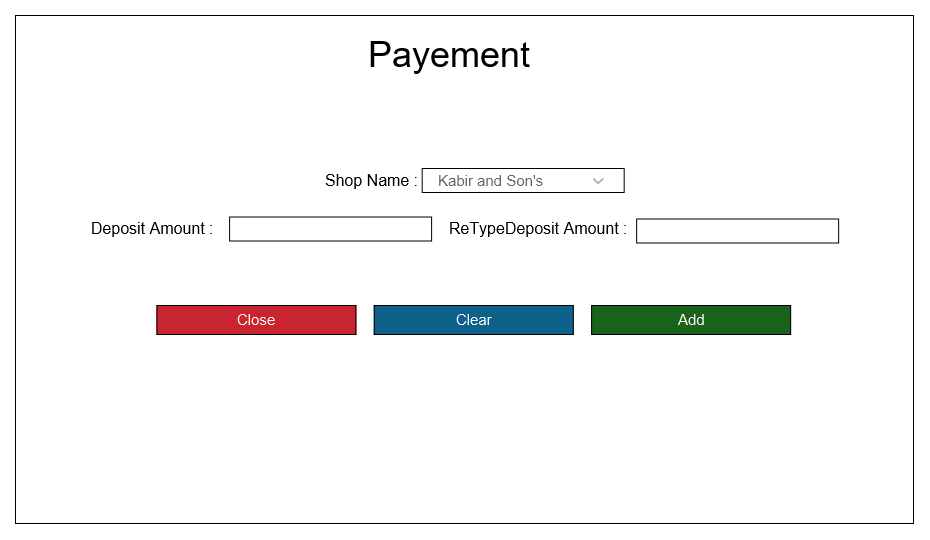
\includegraphics[scale=0.3]{./UIs for Latex Reports/UI-026 Add Payment@1x.png}\end{center}  \\ \hline

Validators & 
\begin{itemize}
\item   Deposit and Retype Deposit Amount must be a number not string
\item  Before Clicking Add, Both fields must be filled
\item  Both fields must be same


\end{itemize}
\\ \hline

\end{tabular} 
%------------------------------------------
\section{Withdraw Expenses }

\begin{tabular}{ | m{3cm} | m{12cm}| } \hline

Interface ID & I26  \\\hline

Name  & Withdraw Expenses  \\ \hline

Linked Use Case &  \\ \hline

UI Interface in JUSTINMIND & \begin{center} 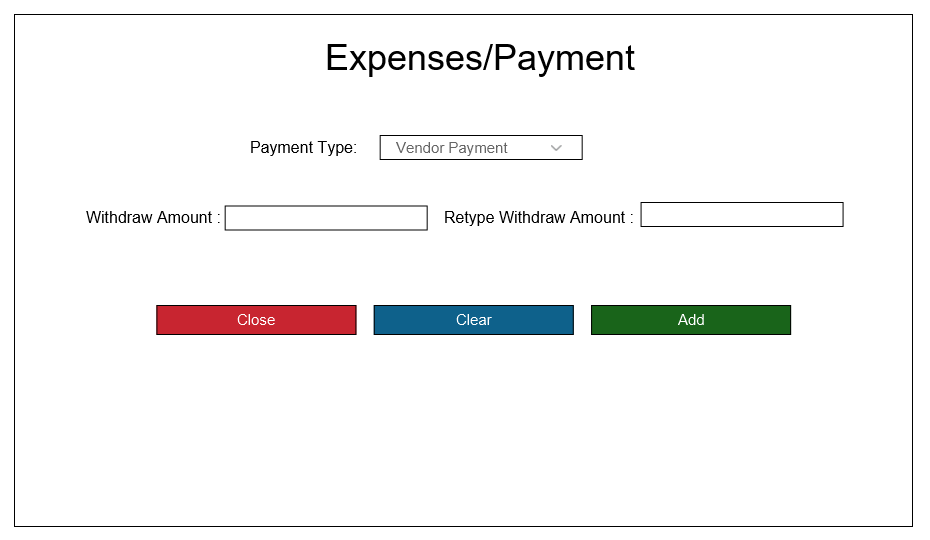
\includegraphics[scale=0.3]{./UIs for Latex Reports/UI-027 Add Withdraw Expenses@1x.png}\end{center}  \\ \hline

Validators & 
\begin{itemize}
\item   Withdraw and Retype Withdraw Amount must be a number not string
\item  Before Clicking Add, Both fields must be filled
\item  Both fields must be same


\end{itemize}
\\ \hline

\end{tabular} 
%------------------------------------------
\newpage
\chapter {User Interface Details }
\begin{center}
\begin{tabular}{ | m{1.5cm} | m{1.5cm}| | m{1.5cm}|| m{1.5cm}| | m{1cm} | m{1.5cm}| | m{1.5cm}|} 
 \hline
\textbf{ Interface Id} & \textbf{Text Box} & \textbf{Drop Down} & \textbf{Password Box} & \textbf{Table} & \textbf{Date Field} &\textbf{Buttons} \\  \hline
  101 &0 & 0 & 0 & 0 & 0 & 0 \\ \hline
  102 &1 & 1 & 1 & 0 & 0 & 3 \\ \hline
  103 &1 & 1 & 2 & 0 & 0 & 3 \\ \hline
  104 &5 & 1 & 2 & 0 & 0 & 3 \\ \hline
  105 &5 & 1 & 2 & 0 & 0 & 3 \\ \hline
  106 &1 & 3 & 0 & 1 & 0 & 5 \\ \hline
  107 &0 & 0 & 0 & 1 & 0 & 0 \\ \hline  
  108 &13 &1 & 0 & 0 & 0 & 3 \\ \hline  
  109 &13 &0 & 0 & 0 & 0 & 3 \\ \hline  
  110 &1 & 3 & 0 & 1 & 0 & 5 \\ \hline  
  111 &4 & 4 & 0 & 1 & 0 & 4 \\ \hline
  112 &6 & 0 & 0 & 1 & 0 & 3 \\ \hline  
  113 &2 & 1 & 0 & 0 & 0 & 3 \\ \hline
  114 &8 & 1 & 0 & 0 & 0 & 3 \\ \hline
  115 &8 & 1 & 0 & 0 & 0 & 3 \\ \hline
  116 &1 & 3 & 0 & 1 & 0 & 5 \\ \hline
  117 &0 & 0 & 0 & 1 & 0 & 0 \\ \hline
  118 &0 & 0 & 0 & 1 & 0 & 0 \\ \hline
  119 &0 & 0 & 1 & 0 & 0 & 0 \\ \hline
  120 &8 & 1 & 2 & 0 & 0 & 3 \\ \hline
  121 &8 & 1 & 2 & 0 & 0 & 3 \\ \hline
  122 &8 & 0 & 0 & 0 & 0 & 1 \\ \hline
  123 &0 & 6 & 0 & 0 & 0 & 2 \\ \hline
  124 &10& 1 & 0 & 0 & 0 & 3 \\ \hline
  125 &2 & 1 & 0 & 0 & 0 & 3 \\ \hline
  126 &2 & 1 & 0 & 0 & 0 & 3 \\ \hline
\end{tabular}
\end{center}
%---------------------------------------
\newpage
\begin{center}
\begin{tabular}{ | m{1.5cm} | m{1.5cm}| | m{1.5cm}|| m{1.5cm}| | m{1cm} | m{1.5cm}| | m{1.5cm}|}  
 \hline

\textbf{ Interface Id} &\textbf{ AutoComplete} &\textbf{ Radio Button} & \textbf{Check} \textbf{Box} & \textbf{Menu} & \textbf{Text Area} &\textbf{Progress Bar} \\  \hline
101 & 0 & 0 & 0 & 0 & 0	& 1  \\ \hline
102 & 0 & 0 & 0 & 0	& 0 & 0  \\ \hline
103 & 0 & 0 & 0 & 0 & 0 & 0  \\ \hline
104 & 0 & 2 & 0 & 0 & 1 & 0  \\ \hline
105 & 1 & 2 & 0 & 0 & 1 & 0  \\ \hline
106 & 0 & 0 & 0 & 0 & 0 & 0  \\ \hline
107 & 0 & 0 & 0 & 14 & 0 & 0  \\ \hline
108 & 0 & 2 & 0 & 0 & 0 & 0  \\ \hline
109 & 0 & 2 & 0 & 0 & 0 & 0  \\ \hline
110 & 0 & 0 & 0 & 0 & 0 & 0  \\ \hline
111 & 0 & 0 & 1& 0 & 0 & 0  \\ \hline
112 & 0 & 0& 0 & 0 & 0 & 0  \\ \hline
113 & 0 & 0 & 0 & 0 & 1 & 0     \\ \hline
114 & 1 & 0 &0 & 0 & 0 & 0  \\ \hline
115 & 1 &0 & 0 & 0 & 0 & 0  \\ \hline
116 & 0 & 0 & 0 &0 & 0 & 0  \\ \hline
117 & 0 & 0& 0 & 10 & 0 & 0  \\ \hline
118 & 0& 0 & 0 & 14 & 0 & 0  \\ \hline
119 & 0 & 0& 0 & 11 & 0 & 0  \\ \hline
120 & 0 & 2 &0 & 0 & 0 & 0  \\ \hline
121 & 1& 2 & 0 & 0 & 0 & 0   \\ \hline
122 & 0 & 2& 0 & 0 & 0 & 0  \\ \hline
123 & 0 & 0 & 0 & 0 & 0 & 0  \\ \hline
124 & 0 & 2& 0 & 0 & 1 & 0   \\ \hline
125 & 0& 0 & 0 & 0 & 0 & 0  \\ \hline
126 & 0 & 0& 0 & 0 & 0 & 0  \\ \hline
\end{tabular}
\end{center}
%------------------------------------
\newpage
\chapter {Classes}
The classes which are used in the project are as under with there specific properties. 
\begin{center}
\begin{tabular}{ | m{4cm}|m{4cm}|m{4cm}|} 
 \hline

\textbf {Class Name} & \textbf{ Software/ Domain }&\textbf {Is Abstract (Yes/No)}\\ \hline
 CEO 		&Domain			&No\\ \hline
Company		&Domain			&No\\ \hline
Office		&Domain			&No\\ \hline
WareHouse	&Domain			&No\\ \hline
User		&Domain			&No\\ \hline
Rider		&Domain			&No\\ \hline
Employee  	&Domain			&No\\ \hline
WareHouseManager&Domain		&No\\ \hline
ShopOwner 	&Domain			&No\\ \hline
Shop	  	&Domain			&No\\ \hline
Ledger	  	&Domain			&No\\ \hline
Order		&Domain			&No\\ \hline
Product		&Domain			&No\\ \hline
Vehicle		&Domain			&No\\ \hline
Stack		&Software		&No\\ \hline
Queue		&Software		&No\\ \hline
Linked List	&Software		&No\\ \hline
Binary Search Tree&Software	&No\\ \hline
\end{tabular}
\end{center}
%----------------------------
\begin{center}
\begin{tabular}{ | m{4cm}|m{4cm}|m{4cm}|} 
 \hline

\textbf{ Class Name} &\textbf{ Is Singleton (Yes/No)} &\textbf {Is the class will has parametrized constructor(Yes/No)}\\ \hline
 CEO 		&Yes	&Yes \\\hline
Company		&Yes	&Yes \\\hline
Office		&Yes	&Yes \\\hline
WareHouse	&No		&Yes \\\hline
User		&No		&Yes \\\hline
Rider		&No		&Yes \\\hline
Employee  	&No		&Yes \\\hline
WareHouse Manger  &No		&Yes\\ \hline
ShopOwner 	&No		&Yes\\ \hline
Shop	  	&No		&Yes \\ \hline
Ledger	  	&Yes	&Yes \\ \hline
Order		&No		&Yes \\ \hline
Product		&No		&Yes \\ \hline
Vehicle		&No		&Yes \\ \hline
Stack		&No		&Yes \\ \hline
Queue		&No		&Yes \\ \hline
Linked List	&No		&Yes \\ \hline
Binary Search Tree  &No		&Yes\\  \hline
\end{tabular}
\end{center}
%------------------------------------
\newpage
\chapter {Object Oriented Features}
\section{Composition}
In our Project there are 8 places where we use Composition
\begin{itemize}
\item   Company Class has composition of Ledger Class
\item  Company Class has composition of Office Class
\item  Company Class has composition of Warehouse Class
\item  Company Class has composition of CEO Class
\item  Warehouse Class has composition of  Warehouse Manager Class
\item  Rider Class has composition of Vehicle Class
\item  Office Class has composition of User Class ( Employee, Rider)
\item  Shop Owner Class has composition of Shop Class
\end{itemize}
\section{Inheritance}
In our project inheritance is used in following places
\begin{itemize}
\item   User inherits the class of CEO
\item User inherits the class of Rider 
\item User inherits the class of Shopkeeper
\item User inherits the class of Warehouse Manager  
\end{itemize}
\section{Multi-Level Inheritance}
In our project Multilevel inheritance is used as
\begin{itemize}
\item User class inherits the CEO class and CEO class inherits the Employee Class
\end{itemize}
\section{Aggregation}
In our project Multilevel inheritance is used as
\begin{itemize}
\item Rider Aggregate the Rating Class in our project
\end{itemize}
\section{Association}
In our project Multilevel inheritance is used as
\begin{itemize}
\item Warehouse Manager manages the order.
\item CEO manages the products
\item Rider take the order 
\item Rider adds the order
\item Employee adds the products
\item Employee manages the order 
\end{itemize}


\newpage
\chapter {Detailed Object Oriented Design}

\begin{figure}
  \centering
    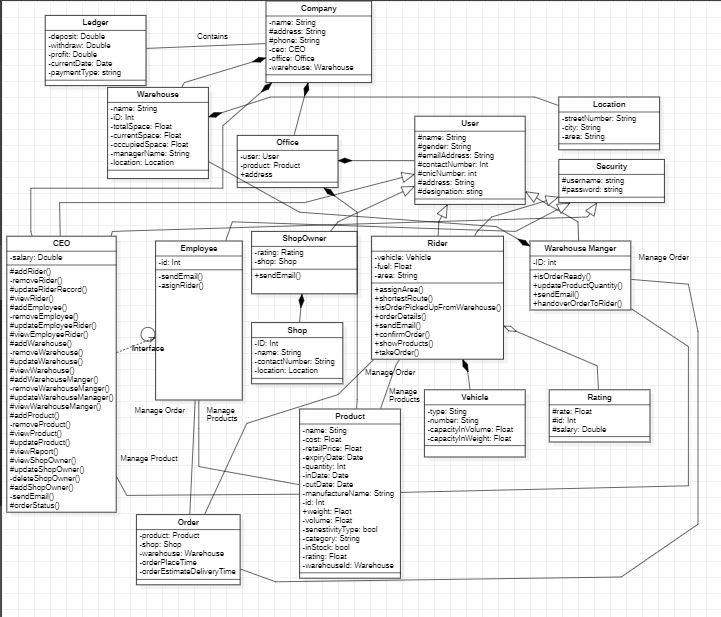
\includegraphics[scale=0.8]{./UIs for Latex Reports/UML.jpg}
  \caption{The detailed Object Oriented Design of the project that will be implemented according to mentioned logic}
\end{figure}
\newpage
\chapter {Data Structure}

\begin{tabular}{ | m{2cm} | m{3cm}|m{9cm}| } \hline
\textbf{ Use Case ID}&	\textbf{Data Structure Used}	& \textbf{Justification for the use of data structure}  \\ \hline
U01 &Linked List& In the U01 (LOGIN), search and compare the user from the list so when the user data is found it returns the action.\\ \hline
U04 &Linked List& In the U04 (Account Details), Grid of the added users shown lists where all the users are stored(added) \\ \hline
U05 &Linked List& In the U05 (Update Account), Update data of  the user present in the Linked List\\ \hline
U06 &Linked List&In the U06 (Add Product), Add the product data in the List. \\ \hline
U07 &Linked List&In the U07 (View Product), View the product data in the Grid that are stored in the list at the backend. \\ \hline
U08 &Linked List& In the U08 (Update Product), Update the product data in the list where the data of the products are added.\\ \hline
U09 &Linked List& In the U09 (Add Rider), Add the Rider data in the List. Selection of the list is because there is the ease in the deletion and search in the data of list\\ \hline
U10 &Linked List&In the U10 (Update Rider), update the rider data. Selection of the list is to search is to ease. \\ \hline
U11 &Queue      & In the U11(Order Product), To place the order we use the mechanism of First in and First Out (first order item will be placed first)\\ \hline
U12 &Stack      & In the U12 (Email), To send the mail and view the mail (first send mail is shown in the last and the most recent one in the first)\\ \hline
U13 &Linked List& In the U13 (Add Warehouse), Add the detail data of the warehouse in the list.\\ \hline
\end{tabular}
\begin{tabular}{ | m{2cm} | m{3cm}|m{9cm}| } \hline
U14 &Linked List& In the U14 (Detail Warehouse), Select the desired warehouse and delete the data of the warehouse and also delete the data from the list and selection of list is that to delete the warehouse other indexes of list easily manage.
 
\\ \hline
U15 &Linked List&In the U15 (Edit Warehouse), Select the data from the list and Edit the detail data of the warehouse in the list. 
 
 \\ \hline
U16 &Linked List& In the U16 (Order Status), Data is selected and data of the desired Order is updated in the list.\\ \hline
U17 &BST        & In the U17 (Route Finder), Routes are found according to the points (nodes) so selection of BST is due to the ease of the data finding.\\ \hline
U18 &Linked List&In the U18 (Add Shopkeeper), Add the shopkeeper data in the list because there is an ease for the deletion and searching. \\ \hline
U19 &Linked List& In the U19 (Add Payment), payment of the specific shopkeeper is added on the list to search and edit the details in the list.\\ \hline
U20 &Linked List&In the U20 (Add Expenses Amount), Add the Expenses data in the List. Because there is an ease to update the specific data in the list and search or delete it in list. \\ \hline
U21 &Linked List&In the U21 (Create Account), Linked list is used to add user. \\ \hline

\end{tabular}
\newpage
\chapter {Exceptions}

\begin{tabular}{ | m{2cm} | m{5cm}|m{3cm}||m{4cm}| } \hline
\textbf{Type of Exception} & \textbf{Why this exception will occur} &\textbf{ Use Case Id in which exception could be occurred} & \textbf{How you will handle the} exception \\  \hline
Incorrect Format&By default system, take all input in string and the deploy system need to convert into desire format. If the input data is not converted into other datatype like int and float the future task not performed e.g. string 2 and int 2 behave different in CPU. &U06,U19,U09&Restrict the user to enter the required data in correct format.                      \\  \hline
File not Exit &The required file not in the correct path and CPU not recognize it.&U14,U07,U04&Restrict the user first select the file then perfrom future action
\\  \hline
Incorrect URL& The wrong URL of the website broken the link with the DNS and required data not fetch from server. &U17&Apply stick constrain to avoid it. \\
\hline

\end{tabular}
\newpage
\chapter {Data Storage}

\section{Mails (CSV)}
Columns data names are
\begin{enumerate}
\item Columns data names are
\item Employee and Rider
\item Rider and Shopkeeper
\item Warehouse Manager and Employee
\item CEO and Employee
\end{enumerate}


\section{Products (CSV)}
Columns data names are
\begin{enumerate}
\item Name
\item Cost
\item Retail price
\item Expiry Date
\item Quantity
\item In date 
\item Out date
\item Manufacturer 
\item ID
\item Weight
\item Volume
\item Category
\item Sensitivity
\item In stock
\item Rating
\item Warehouse Hold ID
\end{enumerate}

\section{Users (CSV)}
Columns data names are
\begin{enumerate}
\item Name 
\item Gender
\item Email address
\item Contact Number
\item CNIC number
\item Address
\item Desigination 
\end{enumerate}

\newpage
\chapter {Email Sending}
At first
\begin{enumerate}
\item Rider will email the employee about the order of shopkeeper
\item Employee email warehouse manager to ready the shipment for rider
\item Rider will email the Employee and Shopkeeper that he has picked the order and cc to CEO.
\end{enumerate}

\newpage
\chapter {Project Plan}
\begin{tabular}{ | m{2cm} | m{4cm}|| m{3cm}|} \hline
\textbf{ Use Case Id }&\textbf{ Member Name}&\textbf{Estimated Completion Date} \\ \hline
001-008& Syed Hashir 	&09/12/2022   \\ \hline
009-018& Kabir Ahmed	&10/12/2022   \\ \hline
019-026& M. Hamad Hassan&11/12/2022  \\ \hline
\end{tabular}


\newpage
\chapter {Analytical Reports}
In our project, we can use the analytical reports
\begin{enumerate}
\item Salary Report  
\item Rider Capture Order Report 
\item Profit Report 
\item Sold Products


\end{enumerate}


\end{document}


